\documentclass[
    % -- opções da classe memoir --
    12pt,               % tamanho da fonte
    openright,          % capítulos começam em pág ímpar (insere página vazia caso preciso)
    %twoside,            % para impressão em verso e anverso. Oposto a oneside
    oneside,
    a4paper,            % tamanho do papel. 
    % -- opções da classe abntex2 --
    %chapter=TITLE,     % títulos de capítulos convertidos em letras maiúsculas
    %section=TITLE,     % títulos de seções convertidos em letras maiúsculas
    %subsection=TITLE,  % títulos de subseções convertidos em letras maiúsculas
    %subsubsection=TITLE,% títulos de subsubseções convertidos em letras maiúsculas
    % para pacote url reconhecer hifens como separador
    hyphens,
    paginasA3,  % indica que vai utilizar paginas em A3 
    GLOSSARIO, % gerar glossario a partir do arquivo defs-glossario.tex
    TODO, % indica que deve apresentar lista de pendencias 
    % -- opções do pacote babel --
    english,            % idioma adicional para hifenização
    brazil           % o último idioma é o principal do documento
    ]{ifsp-spo-inf-ctds} % ajustar de acordo com o modelo desejado para o curso

% ---
% Informações de dados para CAPA e FOLHA DE ROSTO
% ---
\titulo{STUDY FLOW}

% Trabalho em Equipe
% ver também https://github.com/abntex/abntex2/wiki/FAQ#como-adicionar-mais-de-um-autor-ao-meu-projeto
\renewcommand{\imprimirautor}{
\begin{tabular}{lr}
Kevin Klein & SP3096289 \\
Leonardo Tumani & SP309474X \\
Luiz Fernando & SP3096301\\
Ruan de Souza  & SP3069672 \\
Pedro Dias & SP3099211 \\
\end{tabular}
}


\disciplina{PI1A5 - Projeto Integrado I}

\preambulo{Desenho da aplicação para disciplina de PI1A5}

\data{2024}

% Definir o que for necessário e comentar o que não for necessário
% Utilizar o Nome Completo, abntex tem orientador e coorientador
% então vão ser utilizados na definição de professor
\renewcommand{\orientadorname}{Professor:}
\orientador{JOHNATA SOUZA SANTICIOLI}


% ---


% informações do PDF
\makeatletter
\hypersetup{
        %pagebackref=true,
        pdftitle={\@title}, 
        pdfauthor={\@author},
        pdfsubject={\imprimirpreambulo},
        pdfcreator={LaTeX with abnTeX2 using IFSP model},
        pdfkeywords={abnt}{latex}{abntex}{abntex2}{IFSP}{\ifspprefixo}{trabalho acadêmico}, 
        colorlinks=true,            % false: boxed links; true: colored links
        linkcolor=blue,             % color of internal links
        citecolor=blue,             % color of links to bibliography
        filecolor=magenta,              % color of file links
        urlcolor=blue,
        bookmarksdepth=4
}
\makeatother
% --- 

% carregando aqui referencias quando utilizando BIBLATEX
\IfPackageLoaded{biblatex}{%
\addbibresource{referencias.bib}
}{}

% ----
% Início do documento
% ----
\begin{document}



% Retira espaço extra obsoleto entre as frases.
\frenchspacing 

%somente para o exemplo, fica primeiro
% \todo[inline]{Remover texto informativo inicial}
% \newcommand{\urlmodelosimples}{https://www.sharelatex.com/project/58a3a66af9bb74023ba1bd56}

\newcommand{\urlmodelo}{\url{\urlmodelosimples}}

Esse documento foi feito a partir do modelo canônico do \abnTeX, o acesso ao PDF pode ser feito em 
\urlmodelo. A estrutura utilizada aqui foi um modelo utilizado no curso de Pós Graduação em Gestão de TI do \ac{ifsp}.
\todo{Remover texto informativo inicial}

%%A versão do sharelatex atualmente é a mais atualizada

%A versão atualizada da classe \ac{ifsp} para \LaTeX pode ser acessada em %\url{https://github.com/ivanfmartinez/latexlib/tree/master/ifsp}.

Este documento não pode ser considerado como um padrão a ser seguido em sua totalidade, ele tem como maior objetivo demonstrar como utilizar o \LaTeX para obter um documento atendendo ao máximo o padrão do \ac{ifsp} e \ac{abnt}.



\noindent\hrulefill



\newpage


% -- lista de pendencias gerada pelo todonotes
% -- altere opções do usepackage para remover na versão final....
% \listoftodos
% \todo[inline]{remover lista de todo da versão final...}
\newpage

% ----------------------------------------------------------
% ELEMENTOS PRÉ-TEXTUAIS
% ----------------------------------------------------------
\pretextual

% ---
% Capa
% ---
% \imprimircapa

\newcounter{todocounter}
\newcommand{\todonum}[2][]
{\stepcounter{todocounter}\todo[#1]{\thetodocounter: #2}}

\imprimirfolhaderosto

% ---
% inserir lista de ilustrações
% ---
%\pdfbookmark[0]{\listfigurename}{lof}
%\listoffigures*
%\cleardoublepage
% ---

% ---
% inserir lista de tabelas
% ---
%\pdfbookmark[0]{\listtablename}{lot}
%\listoftables*
%\cleardoublepage
% ---

% ---
% inserir lista de quadros
% ---
%\pdfbookmark[0]{\listofquadrosname}{loq}
%\listofquadros*
%\cleardoublepage
% ---

%% ---
% inserir lista de símbolos
% ---
\begin{simbolos}
  \item[$ \Gamma $] Letra grega Gama
  \item[$ \Lambda $] Lambda
  \item[$ \zeta $] Letra grega minúscula zeta
  \item[$ \in $] Pertence
\todo[inline]{ajustar utilizando glossaries}
\end{simbolos}
% ---

%\todo[inline]{Remover lista de simbolos se não for necessário}


% ---
% inserir o sumario
% ---
\pdfbookmark[0]{\contentsname}{toc}
\tableofcontents*
\cleardoublepage
% ---


% ----------------------------------------------------------
% ELEMENTOS TEXTUAIS
% ----------------------------------------------------------
\textual


\chapter{Introdução}

\justificativa{No Brasil, temos um importante instrumento de ascensão social através dos estudos, chamado “Concurso Público”. Muitas pessoas se dedicam para essa prova, pois através dela pode-se ter melhores ganhos e estabilidade financeira, além de depender do concurso um emprego sem demissão e plano de carreira atrativo. Com esse cenário, milhares de brasileiros tentam todos os anos a prova para esses concursos públicos para diferentes cargos e diversas esferas do poder público, mas com toda essa gama de provas e quantidade de concorrentes, como se preparar da melhor forma?}

Em nosso país, temos um mercado com grande potencial de crescimento e quando falamos de serviços para “concurseiros” (pessoas que prestam concursos públicos). Os serviços que tem a maior atratividade e público, são as plataformas de ensino direcionado para esse tipo de público. Com a Pandemia de COVID-19 iniciada em 2020, essas plataformas tiveram uma mudança em seu modelo de negócio, precisando se adaptar ao modelo online de educação ou EAD. 

Essa mudança no modelo de negócios das empresas do nicho de educação para concurso público, impactou os seus clientes, que agora consomem em maior quantidade serviços de educação online, aumentando ainda mais a possibilidade de novos serviços para esse tipo de cliente.

Com a migração de cursos antes no presencial, para agora online, os estudantes economizam tempo de deslocamento até a escola, tendo o serviço de aula na palma das mãos. E o tempo é justamente o ativo mais difícil para um estudante de concurso público, pois ele precisa conciliar suas atividades cotidianas e ainda seguir uma rotina de estudos e para iniciantes nesse mundo de concursos, além de tempo o que e como estudar se torna uma dificuldade maior ainda.

A tecnologia é uma grande aliada dos estudantes para ajudar a administrar esse cenário. Com o avanço de tecnologias de Inteligência Artificial, o que antes era um estudo e uma rotina sem parâmetros, pode ser otimizado e organizado de maneira muito mais fácil com a chegada desse recurso.


%Para criar uma sessão
\section{Objetivo}

Este projeto tem como objetivo ajudar os estudantes de concurso público a se organizarem com as matérias e rotina de estudos para um concurso público com o auxĺlio de tecnologias de Inteligência Artificial.

A plataforma em ambiente WEB permitirá que os estudantes enviem o edital em o qual irão prestar a prova e a partir desse edital a plataforma gere uma rotina de estudos personalizada pensando no maior ganho em sua jornada de estudos.

\end{itemize}

\section{Princípios norteadores}

\begin{itemize}
    \item Estimular a autonomia para pesquisa, organização das informações e tomada de decisão;
    
    \item Emular o mundo do trabalho e as dinâmicas do trabalho em equipe;
    
    \item Liberdade de escolha de metodologias, plataformas e tecnologias, desde que justificadas e previamente aceitas pelos professores da disciplina;
    
    \item Oferecer um ambiente seguro para experimentação, erro e aprendizado.
    
\end{itemize}

\todo[inline]{De alguma forma podemos indicar aqui que os projetos podem ser integrados com outras disciplinas desde que os professores concordem e que as avaliações são efetuadas de forma independente a partir dos critérios de cada disciplina}

\section{Visão geral do projeto}

A aplicação a ser desenvolvida deve resolver um problema real, pode ser uma aplicação nova ou também uma evolução ou módulo para uma aplicação já existente de código aberto ou que esteja no repositório de controle de versão.

Essa aplicação pode ser desenvolvida em qualquer plataforma ou linguagem de desenvolvimento desde que compatível com o objetivo (ex uma aplicação para controle de lista de compras não pode ser desenvolvida somente para desktop) e os requisitos apresentados neste documento. A aplicação deve atender aos requisitos apresentados no \autoref{requisitos-aplicacoes}.

\todo[inline]{Precisamos deixar claro aqui a questão dos processos}



\section{Papéis e responsabilidades}

Na disciplina existem diversos papéis que são assumidos pelos participantes, o entendimento desses papéis permite atingir corretamente os objetivos da disciplina:
\begin{itemize}
    \item \textbf{Estudante} - Deve desenvolver as atividades da disciplina seguindo os preceitos deste documento e orientações passadas pelos professores, colaborando para o sucesso do projeto desenvolvido pela equipe;


    \item \textbf{Equipe} - Segundo \cite{EQUIPES}: 
    \begin{citacao}“Um grupo de pessoas com alto grau de interdependência está direcionado para a realização de uma meta ou para a conclusão de uma tarefa, cria-se o conceito de EQUIPE. Em outra palavras, membros de uma equipe concordam com uma meta e concordam que a única maneira de alcançar essa meta é trabalhar em conjunto". 
    \end{citacao}
    Desta forma, as equipes são compostas por um número definido de estudantes, que tem como objetivo a concretização do trabalho da disciplina.
    
    Algumas outras definições de equipes e vídeos de apoio podem ser encontrados em: \dicasIvan{equipes}
    

    \item \textbf{Professor} - Tem o papel de orientar e avaliar, buscando atingir os objetivos da disciplina;
    
    \justificativa{Eles precisam buscar informações antes de nos questionar e vamos atender de acordo com requisições, não devemos influenciar nas decisões se não formos questionados ou consultados}
    

    \item \textbf{Cliente} - Os professores assumem o papel de cliente do projeto e devem ser consultados como um cliente real. Ao desenvolver uma aplicação para resolver um problema real e tendo acesso a usuários reais o projeto pode evoluir muito pois passa por diversas visões em relação ao problema. Uma equipe também pode assumir o papel de cliente de outra equipe desde que não entrem em conflito com as decisões dos clientes principais que são os Professores;

    \item \textbf{Banca Examinadora} - O trabalho é apresentado para uma banca que vai avaliar tanto os documentos demonstrando o desenvolvimento como a aplicação em execução. Essa banca é composta pelos professores da disciplina e convidado(s).
    
\end{itemize}


\section{Avaliações}

Todos as atividades desenvolvidas durante o projeto são avaliadas pelos professores, prazos de entregas são considerados como datas de Provas / Avaliações tradicionais e portanto devem ser respeitados.

Além da documentação e da execução da aplicação, são avaliados os modelos estáticos e dinâmicos da aplicação, bem com a relação entre modelos, aplicação e objetivos do projeto.

A divisão das atividades desempenhadas por cada elemento da equipe deve ser documentada no trabalho. A avaliação pode ser individualizada, conforme as atividades desempenhadas por cada aluno ao longo do projeto.

Cada equipe também faz avaliações de seus membros, cada participante avalia todos os membros de sua equipe (incluindo ele mesmo). Essas avaliações também poderão ser consideradas pelos professores ao definir a nota individual de cada participante.




\section{Comunicação entre alunos e professores}
Existem diversos canais de comunicação que poderão ser utilizados durante o desenvolvimento da disciplina, conforme a seguir descrito.
\begin{itemize}
    \item Comunicador do \ac{suap} onde os professores muitas vezes enviam comunicados oficiais que precisam de registro;
    
    \item Curso definido no Moodle da disciplina onde algumas atividades devem ser entregues e também permite o envio de mensagens;
    
    \item E-mail dos alunos para os professores com dúvidas especificas (sempre enviar com cópia para ambos professores e indicar claramente qual a turma/equipe que faz parte, pois os professores tem projetos de diversas turmas e nem sempre os e-mails chegam com o nome correto do aluno);
    
    \item Grupo no Telegram que permite a comunicação entre todos participantes da turma, dúvidas genéricas devem ser feitas principalmente por esse canal pois permitem que todos tenham acesso a informação. Nesse grupo são enviados os links para as aulas/conversas síncronas da disciplina;
    
    \item Ferramentas de conferencia (Meet, RNP, Teams, Telegram  etc) para conversas síncronas.
    
\end{itemize}

É importante lembrar que algumas ferramentas devem ser utilizadas com cuidado, não se deve enviar mensagem com notificação de madrugada por exemplo. No Telegram é possível agendar o envio de uma mensagem ou até enviar sem a notificação, bastando escolher isso no momento do envio.

Existe um canal genérico de projetos (IFSP-SPO-Projetos) onde algumas informações gerais que atendem alunos do ensino médio e superior são publicadas \url{https://t.me/joinchat/AAAAAET-oEt6v2nyhgx2CQ}.





\justificativa{O Telegram não dá acesso ao número de telefone se o usuário não desejar, assim respeita um pouco o que a própria escola faz onde não temos acesso aos números, os grupos tem o histórico disponível e assim os alunos tem acesso ao que já aconteceu}





% \chapter{Fases da disciplina}
\label{fases-da-disciplina}
Neste capítulo são apresentadas as fases e tarefas do projeto. Todas as atividades são avaliadas pelos professores durante o período da disciplina e não somente nas entregas. 
As datas de entregas podem ser encontradas no plano de aulas disponível no \ac{suap}.

\todo[inline]{Esse capitulo 2 e 3 parecem pequenos e muitas das coisas estão indicadas nos outros, talvez unificar fique melhor : Ivan}

\todo[inline]{Precisamos ajustar aqui as semanas / referencias de acordo com o que definirmos no plano de aula}

\section{Primeira fase}
A primeira fase consiste nas etapas de definição da equipe, análise dos projetos e repositórios, elaboração a apresentação de uma proposta inicial de projeto. 

\begin{itemize}
    \item Definição da equipe \atividade{definicao-equipe};
    
    \item Definição do(a) gerente da equipe \atividade{escolha-gerente};
    
    \item Linha de definição dos acessos no mesmo modelo do acessos.txt do repositório \gls{svn} \atividade{acessos};
    
    \item Criação de blog \atividade{criacao-blog};
    
    \item Criação de canal no YouTube \atividade{criacao-youtube};
    
    \item Arquivo equipe.yaml validado com yamlint com as definições e urls do projeto, blog, YouTube etc \atividade{equipe-yaml};
    
    \item Pesquisa e avaliação de projetos anteriores \atividade{avaliacao-projetos-anteriores};
    
    \item Planejamento \atividade{planejamento-projeto};
    
    \item Proposta inicial \atividade{proposta-inicial};
    
    \item Inicio do desenvolvimento do projeto.
\end{itemize}


\section{Segunda fase}
A segunda fase consiste na entrega da prova de conceito e apresentação do desenvolvimento até o momento.

\begin{itemize}
    \item Prova de conceito \atividade{prova-de-conceito};
    
    \item Desenvolvimento do projeto;
    
    \item Apresentação parcial \atividade{apresentacao-parcial}.
\end{itemize}

\section{Terceira fase}
A terceira fase consiste na entrega e apresentação da primeira versão e análise dos projetos das outras equipes.

\begin{itemize}
    \item Entrega primeira versão \atividade{primeira-versao};

    \item Apresentação primeira versão \atividade{apresentacao-primeira-versao};
    
    \item Acompanhamento das apresentações de todas as equipes e criação de Relatório de análise dos projetos das outras equipes \atividade{relatorio-analise-projetos}.
\end{itemize}

\justificativa{Normalmente aqui vem o ENEM então deixamos essa fase somente para os ajustes...}

\section{Quarta fase}
A quarta fase consiste na verificação dos relatórios de análises dos projetos e sugestões da banca e correções.

\begin{itemize}
    \item Ajustes e finalização da aplicação desenvolvida;
    
    \item Apresentação final do projeto \atividade{entrega-final}.
    
\end{itemize}

\section{Continuamente durante o projeto}

\begin{itemize}
    \item Publicação semanal no blog \atividade{publicacao-blog};
    

    \item A cada apresentação:
      \begin{itemize}
            \item Auto avaliação da equipe \atividade{planilha-notas};
          
            \item \emph{Slides} devem ser colocados no repositório de controle de versão;
          
            \item Vídeo do \gls{gource} \atividade{video-gource}.
      \end{itemize}

       
\end{itemize}



% % \subsubsection{Armadilhas e problemas}
% \subsubsection{Revisão Inicial da Literatura}


\todo[inline]{Uma coisa que sempre pega é deixarem para fazer coisas na ultima hora. Sempre falo no primeiro dia mas não adianta, alguma sugestão ? Gource, latexdiff são processos simples mas precisam baixar os programas e o conhecimento mínimo de executar um comando, muitas vezes ficam apanhando com coisas básicas como espaços nos nomes das pastas, não lerem as mensagens de erro etc....}


% \chapter{Requisitos das aplicações}
\label{requisitos-aplicacoes}

Os requisitos das aplicações estabelecem partes dos critérios de avaliação do componente curricular \ac{pds} e também servem como uma lista de verificação (\emph{checklist}), facilitando a escolha de diferentes soluções e desenvolvimento do projeto.


\section{A aplicação deve resolver problemas dos usuários e tratar processos}

Apesar da possibilidade de resolver alguns problemas reais somente com armazenamento e busca de dados, para as disciplinas de desenvolvimento de projetos é importante o desenvolvimento de atividades / processos dentro da aplicação.

Não é possível determinar um número exato de processos que devem existir dentro de cada aplicação pois existem contextos diferentes, uma determinada aplicação pode ter um processo grande dividido em fases e outra aplicação pode ter um conjunto de pequenos processos sem dependência direta.

Desenvolvimento do \enquote{zero} de funcionalidades que já existem em outras aplicações / bibliotecas não significam o tratamento de um processo na aplicação (ex \emph{chat}, controle de pagamentos, chamadas de \ac{api}) mas a forma que essas funcionalidades são integradas dentro do sistema podem fazer parte de um processo.

Alguns exemplos de itens que são considerados processos :

\todo[inline]{Coisas que o sistema faz para o usuário }
\todo[inline]{\enquote{inteligencia} do sistema }

\begin{itemize}
    \item Gerenciamento de dados entre \enquote{atores} do sistema, com tratamento de permissões responsabilidades;
    
\todo[inline]{talvez colocar exemplos ? }
    
    \item Determinação automática de dados para o usuário (ex utilizar geolocalização para vinculação de dados a locais a partir de histórico de definições do usuário).
\end{itemize}


Alguns exemplos de itens que não são considerados processos (mas que podem fazer parte de processos) :

\begin{itemize}

    \item chamadas simples de \ac{api} ou redirecionamento para outros sistemas (ex chamada de sistema de pagamento externo, envio de mensagem via \ac{api} \gls{rest});

    \item apresentação de dados simples em formato de gráficos, relatórios, \emph{dashboard} sem tratamentos e controles pela aplicação.
\end{itemize}

\todo[inline]{Viabilidade de obtenção de dados, não adianta depender de dados que não podem ser obtidos (ex dados de doenças obtidos por envio pelos hospitais)}

\section{Requisitos aplicáveis a todos os projetos}

Todos projetos devem seguir requisitos gerais que são aplicáveis independente da plataforma utilizada. 

O desenvolvimento deve ser feito utilizando pelo menos uma linguagem orientada a objetos utilizando os conceitos de orientação a objetos.

Encorajamos a utilização de soluções prontas para problemas comuns (autenticação, validação, CRUD etc), lembrem que vocês devem manter o foco na resolução do problema que é o objetivo da aplicação e a tecnologia deve auxiliar vocês nesse objetivo.




\todo[inline]{Seria interessante ter alguma parte onde podemos deixar sugestões que podem ser seguidas ou não dependendo do tipo de aplicação, login social (OAuth  via Facebook, Google, Linkedin etc), login web via Telegram entre outros são bem interessantes e reduzem parte da questão de validação de contas e gerenciamento de senhas de maneira segura}


%\subsection{Legislação, Privacidade e Segurança}

A aplicação deve ser aderente a legislação aplicável (ex LGPD), além de cuidados com critérios de Privacidade, Segurança e Acessibilidade e Performance.

%\subsection{Performance}



\todo[inline]{dados como senhas não devem ser armazenados em texto aberto, mas de forma que possam ser validados sem que os administradores ou qualquer outra pessoa possa obter facilmente}
\todo[inline]{\url{https://owasp.org/www-project-top-ten/}}
\todo[inline]{\url{https://cheatsheetseries.owasp.org/}}


%\todo[inline]{detalhar}
%\dicasIvan{lgpd}

%\subsection{Privacidade}

%\todo[inline]{detalhar}

%\dicasIvan{lgpd}


%\subsection{Segurança}
%\todo[inline]{detalhar}



%\subsection{Acessibilidade}

%\todo[inline]{detalhar}

\subsection{Internacionalização}

Com a globalização e disponibilidade de internet uma aplicação pode ter um alcance mundial, para isso as aplicações devem ser pensadas de forma que possam ser utilizadas em mais de um país, a maioria das linguagens já possuem suporte para isso, seguir os padrões de internacionalização desde o inicio do desenvolvimento permite que facilmente uma aplacação seja adaptada para utilização em diferentes países e linguagens.

A aplicação a ser desenvolvida deve ser acessível na língua portuguesa e mais uma outra língua.

\begin{itemize}
    \item  \url{https://www.w3.org/International/quicktips/index.pt};
    
    \item \url{https://developer.android.com/training/basics/supporting-devices/languages.html}.
\end{itemize}

\todo[inline]{detalhar}


\subsection{Disponibilidade na internet}

A aplicação deve ser disponibilizada para acesso via internet (exceto no caso de aplicação Desktop, para a qual deverá ser disponibilizada a versão distribuível). Existem diversos provedores que oferecem contas gratuitas (AWS, Azure, Google, Oracle Cloud, Heroku etc) e também existe o convenio AWS Educate onde os professores podem disponibilizar uma sala com créditos adicionais para uso dos alunos que solicitarem.

As contas AWS Educate devem ser criadas com o e-mail institucional @aluno.ifsp.edu.br a partir do link disponível em \dicasIvan{ifsp}. Essas contas permitem a criação de maquinas em um Data Center localizado nos Estados Unidos.

Soluções que ficam disponíveis na internet devem ser acessíveis a partir de um nome (via serviço de \ac{dns}) e não somente pelo endereço \ac{ip}. Não existe necessidade de registro de um domínio para isso, pode ser utilizado um serviço de \ac{dns} dinâmico ou mesmo um nome oferecido pelo provedor de hospedagem.

O serviço deve ficar disponível na internet para que o desenvolvimento e testes possam acontecer da melhor maneira possível.


\subsection{Desenvolvimento}

Durante todo o desenvolvimento os requisitos devem ser seguidos:

\begin{itemize}
\item Execução continua de \Gls{analise-estatica} \atividade{analise-estatica};

\item Seguir o \emph{Coding Convention} da linguagem ou definido (e documentado) pela equipe \atividade{coding-convention};

\item Código limpo - \citeonline{clean-code};

\item \Gls{vc} \gls{svn}, seguindo as regras indicadas no repositório\footnote{\url{https://svn.spo.ifsp.edu.br/viewvc/A6PGP/0-LEIA_ME.txt?view=markup}};

\item Preferencialmente utilizar um processo de \Gls{integracao-continua}; 

\item Sistema de log \atividade{log};

\item \Gls{testes} \atividade{testes};

\item \Gls{testes-automatizados} \atividade{testes-automatizados}.

\end{itemize}



\todo[inline]{As aplicações devem ser modeladas de forma compatível com seu objetivo, se uma aplicação tem previsão de crescimento grande os modelos de dados, índices devem ser compatíveis para garantir isso, além da questão de escalabilidade da arquitetura}



\subsection{Volume de dados para demonstração das funcionalidades}
As aplicações devem ser testadas e demonstradas com um volume de dados compatível com seus objetivos e também para demonstrar de forma clara o funcionamento correto. Colocar somente um registro em cada tabela não permite demonstrar funcionamentos básicos de paginação, ordenação, filtros e tempo de acesso.



\section{Requisitos por plataforma}
Uma plataforma é o ambiente específico no qual a aplicação é executada, podendo ser Desktop, Web, Móvel, Embarcado. 



\subsection{Desktop}
Aplicações desktop são softwares utilizados para executar tarefas específicas e podem ser instalados em um único computador. Exemplos de aplicações desktop: Processadores de texto como o Apache OpenOffice Writer e Microsoft Word; Editores de imagem como o Gimp e Adobe Photoshop.

A plataforma desktop deve ser considerada caso a solução tenha elevado nível de interação com hardware e sistema operacional e requisitos altos de segurança e proteção da informação. 

O desenvolvimento para esta plataforma deve ser avaliado com cuidado, pois carrega um conjunto de desafios que já foram resolvidos com as aplicações web e móvel. Dentre os desafios estão: a distribuição e atualização do software; suporte e problemas relacionados ao ambiente; compatibilidade com diferentes sistemas operacionais; e requisitos mínimos de hardware.

Requisitos para a plataforma desktop: 

\begin{itemize}
  \item Definir como será realizada a distribuição do software;
  
  \item Definir licenciamento do software;
  
  \item Garantir compatibilidade com os plataformas e sistemas operacionais definidos nos requisitos não funcionais do projeto;
  
  \item Definir os requisitos mínimos de hardware;
  
  \item Testar os requisitos mínimos de hardware.
\end{itemize}

\subsection{Web}
Aplicações web são softwares utilizados através de um navegador podendo ser disponibilizados por um servidor \ac{http} de forma remota ou localmente no dispositivo do usuário. Exemplos de aplicações web: Sistemas acadêmicos como o SUAP; E-commerce como a Amazon; Redes sociais como Facebook e Instagram.

Em geral, as aplicações web são construídas usando o modelo de solicitação e resposta do protocolo \ac{http}. Neste modelo, o cliente (navegador ou outro software) realiza uma requisição a um servidor que processa e devolve uma resposta. Em seguida, a resposta é tratada e utilizada pelo cliente. 

Para garantir a privacidade neste tipo de aplicação deve ser utilizado o protocolo \ac{https} que é a versão criptografada do \ac{http}.

Dentre os tipos de soluções para a plataforma web estão:  Serviços Web, \ac{mpa}, \ac{spa} e \ac{pwa}.

Os Serviços Web, em geral, não entregam conteúdo de apresentação (\ac{html}, \ac{css}, entre outros formatos). O foco desse tipo de solução é a exposição de funcionalidades e dados para integração entre diferentes partes do sistema ou entre sistemas diversos. Dessa forma, os requisitos gerais para plataforma web a seguir não incluem os requisitos para os serviços web, apenas para as soluções \ac{mpa}, \ac{spa} e \ac{pwa}:

\begin{itemize}
  \item Aplicar as técnicas de layout e conteúdo responsivo\footnote{\url{https://developer.mozilla.org/en-US/docs/Web/Progressive_web_apps/Responsive/responsive_design_building_blocks}};
  
  \item Atender no mínimo os requisitos de nível A das diretrizes de acessibilidade \ac{wcag} disponível em \url{https://www.a11yproject.com/checklist/};
  
  \item Validar código-fonte de apresentação utilizando os serviços indicados a seguir:
  \begin{itemize}
    \item Validador \ac{html} disponível em \url{https://validator.w3.org/};
    
    \item Validador \ac{css} disponível em \url{https://jigsaw.w3.org/css-validator//}.
  \end{itemize}
  
  \item Realizar testes de usabilidade dos principais pontos de interação do software utilizando ferramentas gratuitas; 
  \todo[inline]{Detalhar um pouco mais depois, existem serviços gratuitos que podem ser utilizados.}
  
  \item Bibliotecas javascript, \ac{css} e similares de terceiros que são disponibilizadas via \ac{cdn} não devem ser incluídas diretamente no projeto.  

\end{itemize}

\subsection{Móvel}
O desenvolvimento para plataforma móvel não se limita apenas a smartphones, mas a um conjunto de dispositivos como tablets, relógios inteligentes entre outros. Na plataforma móvel um software é chamado de aplicativo ou \emph{app}. O desenvolvimento de aplicativos pode adotar o modelo nativo, multi-plataforma (\emph{cross-platform}) ou hibrido.

Um aplicativo nativo é aquele desenvolvido de forma exclusiva para um determinado sistema operacional, como o Android ou iOS. Neste modelo, o aplicativo é capaz de consumir diretamente as funcionalidades e recursos do dispositivo e do sistema operacional, tais como câmeras, bluetooth e \ac{gps}. Linguagens de programação como Kotlin ou Java podem ser utilizadas no desenvolvimento Android. Para o sistema operacional iOS são adotadas as linguagens Swift ou Objective-C.

Os aplicativos multi-plataforma (\emph{cross-platform}) permitem gerar executáveis para diferentes plataformas ou sistemas operacionais a partir de uma única base de código. Neste modelo, apenas um aplicativo é desenvolvido e executado em diferentes sistemas como Android e iOS. Isso ajuda as empresas a alcançar um número maior de usuários e também a diminuir o custo com o desenvolvimento e manutenção de versões do aplicativo para diferentes plataformas. Dentre as ferramentas disponíveis para esse modelo de desenvolvimento estão o Flutter\footnote{\url{https://flutter.dev/}} e o React Native\footnote{\url{https://reactnative.dev/}}.

O modelo hibrido consiste um uma mistura de uma solução nativa com uma solução web, escrita com as linguagens \ac{html}, \ac{css} e Javascript dentro de um aplicativo nativo usando um mecanismo de \emph{plugin} como Apache Cordova\footnote{\url{https://cordova.apache.org/}} ou Ionic Capacitor\footnote{\url{https://capacitorjs.com/}}. Esse mecanismo de \emph{plugin} permite o acesso aos recursos nativos das plataformas. No entanto, o grande desafio é conseguir a mesma experiência de interação do usuário que é possível nos modelos nativo ou multi-plataforma.

Requisitos para a plataforma móvel: 

\begin{itemize}
  \item Definir como será realizada a distribuição do software;
  
  \item Definir licenciamento do software;
  
  \item Garantir compatibilidade com as plataformas e versões dos sistemas operacionais definidos nos requisitos não funcionais do projeto;
  
  \item Definir e testar os requisitos mínimos de hardware;
  
  \item Atender os padrões de interação e uso de componentes definidos em recomendações de cada sistema operacional:
  
  \begin{itemize}
      \item Material Design para Android disponível em \url{https://material.io/};
      
      \item Human Interface Guidelines para IOS disponível em \url{https://developer.apple.com/design/human-interface-guidelines/}.
  \end{itemize}
  
\end{itemize}


\subsection{Embarcado}

Aplicações embarcadas são aquelas que são executadas em um hardware dedicado e interagem com recursos do meio ambiente ou sensores. Essas aplicações normalmente são executadas em equipamentos dedicados como Arduino, ESP8266, Raspberry Pi etc.

Essas aplicações normalmente são conectadas a um servidor Web que gerencia os dados e combina características de Desktop, Web e Móvel.

\todo[inline]{O \ac{ifsp} possui alguns kit Arduino que podem ser emprestados para os alunos que tenham projetos de desenvolvimento  nessa plataforma
\newline com ensino remoto isso não esta valendo}


\section{Requisitos por tipo de solução}

Tipos de solução são definidos por plataforma (Desktop, Web, Móvel e Embarcado). Esses tipos herdam as características e requisitos da plataforma e também podem conter requisitos específicos.

Dependendo da solução ou tipo de projeto a ser desenvolvido, podem ser necessários um ou mais tipos de aplicação, cada qual com sua responsabilidade. Por exemplo, uma \acs{spa} normalmente possui uma aplicação front-end (a aplicação com a qual o usuário irá interagir) e um serviço web, com a qual o front-end se comunica. Dessa forma é importante que as técnicas adequadas sejam usadas no desenvolvimento de cada uma dessas aplicações assim como os requisitos necessários sejam obedecidos.




\subsection{Serviços web}
Um Serviço Web é um software desenvolvido para oferecer interação entre sistemas. Eles podem ser criados para utilização por aplicações terceiras ou para divisão de uma mesma aplicação, tornando o sistema mais organizado e isolando todo o processamento da interface com o usuário. 

Uma aplicação desenvolvida com base em serviços pode ter uma interface Desktop, Web ou em dispositivo móvel sem necessitar de grandes mudanças, além de permitir o consumo desses serviços por outras aplicações facilitando a integração.

São considerados requisitos para os serviços web desenvolvidos no decorrer do projeto: 

\begin{itemize}

    \item Documentação de acordo com as práticas relacionadas ao tipo de serviço desenvolvido, devidamente hospedados para consulta online: utilizando o padrão \gls{openapi} 3 em \ac{json} ou \ac{yaml} para serviços web REST, WSDL para serviços SOAP, ou ainda observando as boas práticas e recomendações do formato / modelo utilizado;
    \todo[inline]{ajustar essas siglas}
    
%   \item Documentar o serviço utilizando o padrão \gls{openapi} 3 em \ac{json} ou \ac{yaml}
    \item Validação pelo serviço de todos os dados de entrada, tratando erros e assumindo a possibilidade de requisições inválidas;
    
    \item Controle de acesso por meio de autenticação e se necessário autorização;
    
    \item Deve estar disponível para utilização através da internet até o final da disciplina na semana de IFA;
    
    \item Deve possuir acesso criptografado utilizando \ac{https} \atividade{https};
    
    \item Deve ser acessível utilizando um nome e não por endereço \ac{ip} \atividade{hostname}.
  
\end{itemize}



\subsection{Multi-page application (MPA)}

Aplicações de múltiplas páginas (em inglês "multi-page application", ou \acs{mpa}) são software desenvolvidos para utilização através de um navegador. Em geral, são aplicações desenvolvidas utilizando tecnologias web como \ac{html}, \ac{css} e Javascript, linguagens de programação, \ac{sgbd} e distribuídas por um servidor de \ac{http}.

As \ac{mpa} adotam um projeto de software clássico no qual todo ou a maior parte do conteúdo é construído pelo servidor e devolvido ao navegador. Em geral, para cada interação dos usuários com a aplicação é gerada uma nova requisição ao servidor e recarregamento de página no cliente.

As desvantagens das \ac{mpa} são o acoplamento entre responsabilidades de front-end e back-end. Além disso, a aplicação deste modelo dificulta a estratégia de lançamento de um produto para plataforma web e após validação do mesmo, o lançamento como um app mobile. Neste caso, um serviço web teria que ser construído a partir de uma \ac{mpa}, disponibilizando dessa forma acesso as funcionalidades e dados para o app mobile. 

Requisitos para projetos que possuem soluções de múltiplas páginas são os mesmos definidos para plataforma web.


\subsection{Single-page application (SPA)}

Assim como as \ac{mpa}, as aplicações de página única (em inglês "single-page application", ou \acs{spa}) são softwares desenvolvidos para utilização através de um navegador. No entanto, elas possuem como objetivo principal fornecer uma experiência de interação similar a uma aplicação desktop. Este objetivo é alcançado por meio do carregamento de todo o código necessário na primeira interação do usuário e em seguida o conteúdo é carregado dinamicamente, sem a necessidade de recarregamento da página. 

Em geral, as requisições de conteúdo são realizadas pelo Javascript utilizando variações da técnica conhecida por \ac{ajax}.

Aplicações de página única devem ser consideradas caso a solução necessite de uma experiência de interação de usuário dinâmica, similar a aplicações Desktop e Mobile. Outro requisito que pode direcionar a escolha de uma \acs{spa} é a necessidade de separação das bases de código ou projetos, entre back-end/serviços e front-end, devido a questões de organização da equipe, separação de responsabilidades, tamanho do projeto, segurança ou limitação de acesso.

A escolha de \acs{spa} para aplicações web que usam os buscadores como fonte primária de tráfego, tais como lojas virtuais, blogs e redes sociais com conteúdo público, deve ser feita com cautela. O conteúdo nas \acs{spa} é carregado de forma dinâmica, desta forma, os robôs que fazem a indexação das páginas nos buscadores podem ter acesso somente ao conteúdo inicial e estático, não encontrando páginas internas. Este cenário pode ser resolvido utilizando uma \ac{mpa} pura, ou com uma solução híbrida \ac{mpa} e \ac{spa} (exemplo de loja virtual na qual o catálogo de produtos é uma \ac{mpa} e o carrinho de compras e checkout é uma \ac{spa}).  

Requisitos para projetos que possuem soluções de página única:
\begin{itemize}
  \item Requisitos definidos para plataforma web;
  
  \item Requisitos de cada uma das aplicações envolvidas na construção da solução de acordo com seus respectivos tipos (serviços web, aplicação back-end, aplicação front-end, por exemplo).
  
\end{itemize}


\subsection{Progressive web app (PWA)}

Aplicativos Web Progressivos (em inglês "progressive web app", ou \acs{pwa}) são aplicativos web que usam APIs e recursos dos navegadores, em conjunto com a estratégia de aprimoramento progressivo (em inglês "progressive enhancement") de forma a oferecer uma experiência de usuário semelhante a um aplicativo móvel nativo.

Para considerar uma aplicação web como \acs{pwa} a aplicação deve atender os seguintes requisitos: 

\begin{itemize}
\item Distribuição por meio de rede segura (contextos seguros (\ac{https}));

\item Utilização de \emph{service workers} para interceptação de requisições e implementação de funcionamento \emph{offline}, \emph{cache} e \emph{push notification};

\item Arquivo de manifesto que define informações como nome, ícone e detalhes para que a aplicação web se pareça com um app mobile nativo;

\item Cumprimento dos requisitos de cada uma das aplicações envolvidas na construção da solução de acordo com seus respectivos tipos (serviços web, aplicação back-end, aplicação front-end, por exemplo).

\end{itemize}
 
\subsection{Jogos}

O desenvolvimento de jogos também é permitido desde que realmente seja feito um desenvolvimento e não somente a utilização de uma ferramenta de criação de jogos por meio de um criador e de \emph{scripts}. Nesse caso em cada turma o número de projetos de jogos deve ser inferior a 50\% do total de projetos da turma.

% \chapter{Requisitos de gerenciamento dos projetos}

\todo[inline]{Talvez seja interessante fazer aqui algo parecido com o que foi feito no capitulo 4 \newline, talvez até unificar com o capitulo anterior}

Cada equipe tem liberdade para escolher a metodologia que vai utilizar, mas essas metodologias devem ser seguidas corretamente (ex não tem como utilizar Scrum sem utilizar \emph{sprint}).

O objetivo de uma metodologia de gerenciamento de projetos é, além de organizar o trabalho a ser feito, permitir que haja previsibilidade no que será feito, ou seja, ao surgimento de uma nova demanda ou na ocorrência de um imprevisto (como algum problema com um membro da equipe, ou o aparecimento de um requisito não previsto inicialmente), seja possível que os impactos de tal ocorrência sejam identificados e as devidas medidas para mitigação de seus efeitos sejam tomadas, seja pela reorganização do que precisa ser feito, seja pela determinação de ajustes de escopo do projeto.

Ainda, é possível também que, usando uma determinada metodologia como base, ajustes sejam feitos para que a metodologia se adéque ao dia-a-dia da equipe. Porém é importante que os ajustes feitos sejam devidamente explicados (e documentados) e que tais ajustes não impactem os objetivos na adoção de uma de gerenciamento de projetos.

Independente da metodologia escolhida e dos nomes utilizados em cada uma é importante que exista organização e os artefatos correspondentes de cada metodologia sejam utilizados, como:
\begin{itemize}
    \item Atas;
    
    \item Definição de Papéis e Responsabilidades;
    
    \item Cronogramas;
    
    \item Registro e acompanhamento de métricas;
    
    \item Reuniões.
\end{itemize}

Todos documentos devem ser sempre entregues em formato \ac{pdf} e gerados a partir do \LaTeX.
















% \chapter{Informações sobre as atividades desenvolvidas}

Esse capitulo apresenta as atividades a serem desenvolvidas durante o projeto, as seções em sua maioria seguem a ordem de desenvolvimento. Mas algumas atividades podem acontecer paralelamente a outras, e em alguns casos a preparação para o desenvolvimento da atividade deve ser feito antecipadamente.

\section{Definição da equipe}\label{atv-definicao-equipe}
Os alunos devem se organizar em equipes de acordo com o número definido pelos professores no primeiro dia de aula. Normalmente as equipes variam entre 4 e 6 participantes de acordo com o número de alunos em cada turma. 

\todo[inline]{Aqui a definição do gerente e escolha das equipes seria o ideal, mas nunca aceitam fazer, se tiverem alguma sugestão é interessante colocar}

\todo[inline]{Muitos casos escolhem os amigos e quando um realmente assume o papel de gerente depois deixam de ser amigos.... Quando não estão preocupados vão levando de qualquer forma}

\todo[inline]{a escolha do perfil dos participantes é importante, mas normalmente só escolhem os amigos}



\section{Planejamento do projeto}\label{atv-planejamento-projeto}

Para se obter o resultado desejado e chegar ao objetivo é importante um planejamento adequado e um acompanhamento da evolução desse plano para chegar ao objetivo. Algumas  atividades devem ser executadas de forma sequencial e portanto o planejamento correto evita atrasos pois não adianta colocar mais energia/pessoas para reduzir o tempo de determinadas atividades ou executar paralelamente \cite{brooks1995mythical}.
% Nine people can’t make a baby in a month. (regarding the addition of more programmers to get a project completed faster)



\section{Escolha do(a) gerente da equipe}\label{atv-escolha-gerente}
Cada equipe deve definir um Gerente que deve ser responsável por organizar durante todo o período de desenvolvimento do projeto. O Gerente também é responsável por participar das reuniões de gerencia que podem acontecer durante a disciplina, onde os professores podem passar informações para as equipes.


\section{Envio da linha correspondente ao acessos.txt}\label{atv-acessos}
Para a criação do diretório correspondente da equipe no repositório de controle de versão \atividade{controle-de-versao}, cada equipe deve enviar para os professores uma linha de texto simples (por e-mail) no mesmo formato do arquivo \textbf{acessos.txt} disponível na raiz do repositório de controle de versão. Os prontuários utilizados nesse arquivo devem ser definidos em letras minúsculas, e o acesso ao repositório sempre deve ser feito com login em letras minúsculas.

A maior parte das atividades da disciplina depende do acesso a este repositório, sendo importante que essa atividade seja cumprida no menor tempo para garantir o acesso de todos ao repositório.


\section{Criação de canal no YouTube}\label{atv-criacao-youtube}
Deve ser criado um canal no YouTube para publicação de todos os vídeos gerados durante o desenvolvimento e apresentações do projeto.

\begin{itemize}
    \item todos os vídeos publicados devem ter na descrição e nas tags \textbf{\acs{ifsp}}, \textbf{\acs{spo}} e \textbf{\codigoDisciplina};
    
    \item vídeos do \gls{gource} devem ser publicados nesse canal \autoref{atv-video-gource}.
\end{itemize}

\section{Criação de blog}\label{atv-criacao-blog}
Deve ser criado um blog para a equipe com as seguintes características:
\begin{itemize}
    \item Deve ter um feed \acs{rss} ou Atom, de forma a permitir que as publicações sejam visualizadas na íntegra em ferramentas de consumo destes formatos;
    
    \item O modelo utilizado para o blog deve ser tal que permita a visualização completa de cada publicação, sem necessidade de clicar em um \enquote{ver mais} ou um ícone para permitir a visualização.
    
\end{itemize}

A partir da criação do blog, toda semana deverá ser feita uma publicação de acordo com o descrito na \autoref{atv-publicacao-blog}

A lista de blogs de projetos anteriores está disponível em: \dicasIvan{blogs-de-trabalhos}, muitos desses blogs possuem relatos e dicas que podem auxiliar no desenvolvimento do seu projeto.


\section{Criação e atualização do arquivo equipe.yaml}\label{atv-equipe-yaml}
Deve ser criado um arquivo no diretório da equipe, no repositório de controle de versão, com as informações sobre a equipe e o projeto que vai ser desenvolvido. Esse arquivo deve ser criado a partir da definição da equipe (\autoref{atv-definicao-equipe}) e deverá ser atualizado se houverem mudanças nas informações (ex a primeira versão do arquivo não possui detalhes sobre o projeto a ser desenvolvido, quando o projeto for aprovado pelos professores então o arquivo deverá ser atualizado).

O arquivo deve seguir o mesmo formato dos arquivos já existentes nos diretórios de equipes de projetos anteriores e ser validado com a ferramenta yamllint \url{https://github.com/adrienverge/yamllint} que é utilizada no servidor. Outras ferramentas que possuem o mesmo nome podem ter critérios diferentes de validação então é importante a utilização da ferramenta sugerida.
\justificativa{Muitos alunos tentam utilizar um site com esse nome que não valida da mesma forma e o arquivo acaba sendo recusado.  }

Esse arquivo é a base para definição da página \dicasIvan{blogs-de-trabalhos}, caso a sua equipe não apareça nessa listagem provavelmente o seu arquivo é invalido, e na página existe um link para ver o arquivo combinado que contem as mensagens de erro de validação.

Esses arquivos são processados diariamente para atualização no site.






\section{Documentos do projeto}\label{documentos-latex}

Todos os documentos que serão entregues para avaliação devem ser feitos utilizando o \LaTeX \space de acordo com os padrões da \ac{abnt} e do Guia de Normatização do \ac{ifsp}. Um modelo de documento está disponível em \urlmodelo \space e contem exemplos de diversos itens que normalmente são utilizados nesses documentos. O documento modelo também possui informações sobre procedimentos para revisão dos textos.


No repositório de controle de versão existem documentos de outras equipes que também podem ser utilizados como referência. O documento de modelo também possui informações sobre o desenvolvimento de software e problemas encontrados em projetos anteriores tanto em documentação como em relação ao desenvolvimento. 

Na página \dicasIvan{textos} existem diversas informações uteis para facilitar a elaboração do seu documento. Cuidado com plágio \dicasIvan{plagio}, não faça cópias de outros documentos, escreva com suas palavras e referencie a informação.

A ferramenta overleaf onde o modelo de documento se encontra é uma ferramenta de desenvolvimento de textos \LaTeX, que possui algumas limitações na versão gratuita, é importante que os alunos mantenham um ambiente de compilação em seus computadores de forma a não ficarem dependentes dessa ferramenta \emph{online}. Algumas atividades como a criação do documento de diferenças entre versões \atividade{latexdiff} dependem de um ambiente corretamente configurado e que não funciona diretamente no overleaf. Alguns professores já possuem contas com características adicionais da conta gratuita do overleaf e podem compartilhar projetos com mais recursos, mas isso não deve ser considerado como a solução normal de uso da equipe.
\justificativa{Aqui é importante que aqueles que não tem os recursos ainda compartilhem os seus links de referencia do overleaf para ganharem esse tipo de acesso, acho que são somente 10 referencias para ganhar histórico e compartilhamento ilimitado}


\section{Utilização do repositório de controle de versão}
\label{atv-controle-de-versao}
\todo{Aqui precisa de ajuste para as disciplinas do superior que podem utilizar repositório externo e precisam sincronizar a cada 15 dias}
É obrigatório o uso do repositório de controle de versão indicado pelos professores. A \ac{url} para acesso é disponibilizada no moodle da disciplina. O acesso deve ser feito utilizando como login o prontuário do aluno (spXXXXXX) sempre em letras minusculas. A senha é a mesma que é utilizada para acesso na rede sem fio do Campus e pode ser redefinida no site \url{https://central.spo.ifsp.edu.br/}. O repositório é um sistema de controle de versão centralizado Subversion (informações adicionais em \dicasIvan{subversion}).

O uso correto do repositório permite o desenvolvimento pelos diversos membros da equipe de forma remota mantendo o conteúdo em local de fácil acesso para todos. Os \glspl{commit} devem ser frequentes para garantir que todos tenham acesso ao desenvolvimento atual da equipe, devem seguir as regras indicadas no arquivo \textbf{txt} na raiz do repositório. Cada equipe também deve manter seu próprio \gls{backup} dos dados do repositório.

Cada \gls{commit} deve ter um comentário descrevendo que que foi alterado, essa informação é muito importante também para criação posterior do vídeo com a ferramenta \gls{gource} \atividade{video-gource}.

O Código e documentação de projetos anteriores do curso técnico e superior fica disponível para consulta por todos os alunos do Campus São Paulo do \ac{ifsp}.

A cada entrega/apresentação deve ser feita uma \emph{tag} no repositório indicando a data e tipo de entrega (ex. 2020-02-10-Prova-de-Conceito)\footnote{ \emph{tag} é uma função disponível em sistemas de controle de versão, não significa criar um diretório com o nome indicado}.

Se o projeto a ser desenvolvido for um desenvolvimento de funções adicionais para projeto de código aberto, será permitida a utilização de um repositório externo público após a avaliação e aprovação dos professores. O repositório oficial do \ac{ifsp} deverá ser ser sincronizado pelo menos uma vez a cada 15 dias com a versão atualizada do repositório externo.

\justificativa{No técnico que ainda não tem experiencia continuamos com o repositório centralizado}





\section{Escolha da metodologia de gerenciamento}\label{atv-metodologia-gerenciamento}

Cada equipe tem liberdade para escolha das metodologias utilizadas durante o projeto, para o controle do projeto deve ser escolhida uma (ou combinação de metodologias) de forma a gerenciar a evolução das atividades. É importante que a equipe realmente siga a metodologia escolhida e utilize os artefatos da metodologia.

\section{Escolha da metodologia de desenvolvimento}\label{atv-metodologia-desenvolvimento}

Cada equipe tem liberdade para escolha das metodologias utilizadas durante o desenvolvimento, para o desenvolvimento do software deve ser escolhida uma (ou combinação de metodologias) de forma executar o desenvolvimento. É importante que a equipe realmente siga a metodologia escolhida e utilize os artefatos da metodologia.

\section{Estudo de tecnologias}\label{atv-estudo-tecnologias}

Antes de iniciar o projeto deve ser feito um estudo das tecnologias que podem ser aplicadas no projeto, pequenos programas de teste podem ser desenvolvidos nesse momento para verificar a aderência dessa tecnologia aos objetivos do projeto. Tecnologias já conhecidas reduzem os estudos, mas deve-se tomar cuidado pois existem casos onde mesmo com um novo aprendizado outras tecnologias podem ser mais eficientes para o projeto.

É importante considerar também os custos de determinadas tecnologias ou plataformas. Se o objetivo do projeto é criar uma solução para uma entidade sem fins lucrativos e que não tenha verbas para manter um sistema no ar, não vai adiantar escolher uma plataforma que tenha um custo mensal.
Além disso algumas plataformas tecnologias possuem limites que podem não ser suficientes para o desenvolvimento da aplicação.

O \ac{ifsp} possui convênios que permitem acesso a pacotes de serviços de forma gratuita e também existem programas gratuitos dos grandes provedores de nuvem (ex AWS Educate).
Analisando projetos anteriores \atividade{avaliacao-projetos-anteriores} é possível obter um grande conjunto de ideias sobre tecnologias possíveis de utilização. 



\section{Definição de tecnologias}\label{atv-definicao-tecnologias}

Após o estudo das tecnologias passiveis de aplicação no projeto a equipe deve fazer suas escolhas e desenhar o projeto de acordo com as tecnologias estudadas.
Em alguns casos os provedores de nuvem permitem escolher onde a aplicação será hospedada, Brasil, Europa, América do Norte etc dependendo do tipo de aplicação a localização pode afetar a latência e a experiencia do usuário. 

As escolhas devem ser justificadas e compatíveis com os objetivos do projeto.
\melhorar{complementar mais aqui....}


\section{Proposta inicial}\label{atv-proposta-inicial}
Cada equipe deve elaborar uma proposta indicando a aplicação que deseja desenvolver, a proposta deve ser desenvolvida e apresentada para a turma. Os professores tem que aprovar o tema e o escopo do projeto a ser desenvolvido. É importante que as aulas anteriores sejam utilizadas para apresentar e negociar com os professores as possíveis propostas de forma que, no dia da apresentação, já seja apresentada a versão final acordada com os os professores.


\begin{itemize}

    \item A ordem de apresentação é definida por sorteio;
    
    \item Documento \ac{pdf} gerado no \LaTeX, com aproximadamente 5 páginas de texto contendo contextualização, ideia, objetivos, análise de concorrentes, referências utilizadas a partir da análise de projetos anteriores \atividade{avaliacao-projetos-anteriores} e indicação de tecnologias que pretendem utilizar \atividade{estudo-tecnologias};
    
    \item \emph{Slides} para apresentação da proposta inicial \atividade{slides};
    
    \item Uma apresentação de 10 minutos devera ser feita e será seguida de perguntas/comentários dos professores e alunos da turma;

    \item Vídeo de 5 minutos no YouTube demonstrando essa proposta \atividade{criacao-youtube};
    
    \item Auto avaliação da equipe \atividade{planilha-notas} deve ser entregue no repositório.
\end{itemize}



\section{Definição de coding convention}\label{atv-coding-convention}

A equipe deve definir o padrão de codificação que ira utilizar e seguir durante todo o desenvolvimento de forma que todo o código siga um padrão único. Existem ferramentas de \gls{analise-estatica} que também verificam se o formato do código segue um padrão pré-definido, a utilização dessas ferramentas ajuda a seguir esse requisito de desenvolvimento. 

\section{Modelagem de dados}\label{atv-modelagem-dados}
A modelagem de dados é fundamental para o correto funcionamento de um software. Sendo assim, é importante que a equipe efetue a modelagem correta seguindo o método pertinente ao seu projeto (seja pela utilização de um \ac{mer}, seja pela utilização de um diagrama de classes, quando utilizado um \ac{orm}). Ainda, não basta que seja feita a modelagem, mas que se olhe de forma criteriosa para o modelo gerado e que ele seja validado com dados reais pertinentes à solução proposta.

Uma forma simples de verificar se um determinado modelo de dados atente é fazer exercícios simples de inserção, atualização e exclusão considerando os cenários da aplicação, usando ferramentas simples, como planilhas, e, com base nas informações registradas, tentar \enquote{responder}  a consultas que serão relevantes para seus usuários (observando os requisitos do projeto), de forma a ver se a informação correta será obtida como resposta (e fazendo os devidos ajustes no modelo caso contrário).


\melhorar{falar sobre dados históricos / temporais, eles esquecem coisas básicas como preço que deve ser registrado em uma compra para no futuro saber o valor}

\section{Codificação da aplicação}\label{atv-codificacao-aplicacao}

Durante o desenvolvimento da aplicação diversos critérios devem ser seguidos para garantir que o seu código seja claro tanto para os programadores como para os computadores, os computadores entendem qualquer código que siga os critérios de sintaxe definidos da linguagem, mas as pessoas podem ter dificuldade, a utilização de um mesmo padrão por toda a equipe facilita \atividade{coding-convention}, além da utilização de padrões já existentes de estruturas de dados e de codificação. Isso facilita tanto a manutenção por outras pessoas como também pelo próprio desenvolvedor.

Tenham em mente as seguintes frases\footnote{\url{https://www.javacodegeeks.com/2012/11/20-kick-ass-programming-quotes.html}}:
\begin{itemize}

% https://groups.google.com/g/comp.lang.c++/c/rYCO5yn4lXw/m/oITtSkZOtoUJ?pli=1
    \item \enquote{Always code as if the guy who ends up maintaining your code will be a violent psychopath who knows where you live.} – Martin Golding;
    
    \item \enquote{Any fool can write code that a computer can understand. Good programmers write code that humans can understand.} – Martin Fowler;
    
    \item \enquote{Good code is its own best documentation. As you’re about to add a comment, ask yourself, \textquote{How can I improve the code so that this comment isn’t needed?}} – Steve McConnell.
    
\end{itemize}

\todo[inline]{Buscar as referencias originais}
\todo[inline]{também é um bom local para colocar mais informações do Clean Code}

\section{Criação de ambiente para aplicação}\label{atv-criacao-ambiente}
A partir das escolhas feitas pela equipe \atividade{definicao-tecnologias} deve ser criado o ambiente no provedor escolhido para a aplicação. O ambiente para desenvolvimento e apresentação pode ser uma versão reduzida do ambiente necessário para a aplicação (ex em produção a aplicação precisa de Balanceador de Carga mas para desenvolvimento isso não é necessário). Além disso o ambiente pode ser criado em localização diferente da ideal para redução de custos.
Diferenças entre o ambiente proposto para execução da aplicação e o ambiente utilizado devem ser claramente detalhadas na documentação.
Considerando que os serviços gratuitos possuem limites é possível a utilização de servidores distribuídos entre contas dos membros da equipe. Além disso é importante tomar o cuidado com serviços que fazem cobrança após o limite gratuito de forma a não terem despesas desnecessárias.



\section{Disponibilização da aplicação na internet}\label{atv-hostname}
Para que a aplicação fique disponível na internet deverá ser utilizado um nome de acesso \emph{hostname} em vez de endereço IP. Isso garante que mesmo na mudança do local de hospedagem o endereço de acesso permanece inalterado. Poderá ser utilizado um serviço de \ac{dns} dinâmico (dyndns), endereço oferecido pelo provedor de serviço ou um domínio registrado caso a equipe tenha interesse posterior em manter a aplicação (mas não é necessário o registro de domínio próprio para cumprir os requisitos da disciplina)



\section{Prova de conceito}\label{atv-prova-de-conceito}
Deverá ser desenvolvida uma Prova de Conceito (\ac{poc}) que deve demonstrar a aderência das tecnologias escolhidas com a aplicação que deve ser desenvolvida. Essa prova de conceito deve demonstrar a comunicação desde o usuário até a base de dados e utilizar de forma simples as tecnologias escolhidas para demonstrar que elas funcionam para o objetivo desejado.
\todo[inline]{Alguns não entenderam claramente o que deve entrar na POC, precisamos desenhar melhor....}

\begin{itemize}
    \item Deve ficar disponível de forma pública na internet;
    
    \item Utilizar os ambientes/plataformas escolhidos para implantação \atividade{criacao-ambiente};
    
    \item Comunicação criptografada \atividade{https};
    
    \item Demonstrar o funcionamento da internacionalização (duas línguas), utilizando corretamente as funcionalidades da linguagem a partir de arquivos de recursos com as definições textuais de cada linguagem (não deve ser utilizada tradução de página via Google tradutor);
    
    \item Demonstrar que os dados do usuário são enviados para o servidor e armazenados na base de dados;
    
    \item Demonstrar que APIs especificas atendem as necessidades desejadas;
    
    \item Auto avaliação da equipe \atividade{planilha-notas};
    
    \item Um vídeo de aproximadamente 3 minutos demonstrando a aderência desta prova de conceito com a aplicação final \atividade{criacao-youtube};
    
    \item Um relatório (máximo de 5 páginas) identificando as tecnologias utilizadas e como elas serão utilizadas no projeto (diagrama de arquitetura);
    
    \item Vídeo do \gls{gource} \atividade{video-gource};
    
    \item Uma apresentação de 15 minutos para professores e alunos;

    \item \emph{Slides} \atividade{slides};

    \item A ordem de apresentação é definida por sorteio.
    
    
\end{itemize}

\section{Apresentação parcial}\label{atv-apresentacao-parcial}
A apresentação parcial consiste em mostrar a situação atual do projeto para os professores e alunos das outras equipes, é importante a utilização de um roteiro para demonstrar de maneira eficiente a situação em que o desenvolvimento se encontra tanto em termos de aplicação como de documentação.

\begin{itemize}

    \item Auto avaliação da equipe \atividade{planilha-notas};
    
    \item Vídeo do \gls{gource} \atividade{video-gource};
    
    \item Uma apresentação de 20 minutos para professores e alunos;

    \item \emph{Slides} \atividade{slides};

    \item A ordem de apresentação é definida por sorteio.
    
\end{itemize}





\section{Vídeo do gource}\label{atv-video-gource}
O video criado com a representação do desenvolvimento no controle de versão deve ser feito com a ferramenta \gls{gource} e deve considerar os seguintes itens:

\begin{itemize}
    \item Utilizar opção \textbf{\emph{--key}};
    
    \item Utilizar as opções de legendas (\textbf{\emph{caption}}) para registrar as principais mudanças feitas no repositório;
    
    \item Deve ter aproximadamente 1 minuto para cada bimestre de desenvolvimento;
    
    \item Alterar os \textbf{\emph{userid}} do repositório pelos nomes dos participantes;
    
    \item Colocar uma imagem distinta e especifica para cada usuário;
    
    \item Deve ser publicado no canal do YouTube \atividade{criacao-youtube}.
\end{itemize}

A cada entrega de aplicação e no final de cada bimestre deve ser criado um novo vídeo do \gls{gource}.



\section{Publicação semanal no blog}\label{atv-publicacao-blog}

O blog tem por objetivo servir como registro das atividades realizadas pela equipe a ser acompanhado pelos docentes. Também é importante como memória da equipe, permitindo a consulta pelos membros da equipe de forma a verificar o que ocorreu em uma determinada semana. Dessa forma, é importante considerar o relato do que realmente ocorreu (inclusive pode-se utilizar a publicação combinada a artefatos da metodologia de gerenciamento de projetos utilizada).

A cada semana deve ser publicado no blog pelo menos uma vez indicando as atividades desenvolvidas por cada elemento da equipe. Deve indicar claramente quem foi a pessoa que fez a publicação.

As publicações semanais no blog devem conter um relatório gerencial de andamento do projeto, com identificação do desempenho e das tarefas individuais (ex. reuniões de \emph{milestones}, \emph{project checkpoint}, \emph{sprint review} etc.).


\section{Comunicação criptografada utilizando \acs{https}/\acs{tls}}\label{atv-https}
A comunicação entre os  módulos da aplicação  e usuário devem sempre ser feitas de forma segura. Para isso deve ser utilizado o protocolo \ac{https} ou \ac{tls} que permitem a comunicação de forma criptografada. A configuração pode ser feita utilizando um certificado gratuito como o disponibilizado pelo serviço Let's Encrypt ou também utilizando serviços gratuitos como CloudFare, CloudFront etc.

A configuração desse serviço deve ser avaliada e obter uma nota mínima \textbf{A} \autoref{atv-ssllabs}

\section{Avaliação da configuração \acs{https}/\acs{tls}}\label{atv-ssllabs}

É importante garantir a confidencialidade entre o usuário e a aplicação no servidor, para isso deve ser utilizado um protocolo de criptografia, o mais utilizado é o \ac{https} que pode ser configurado com um certificado gratuito como Let's Encrypt, AWS ou similar ou através de um serviço que já ofereça esse acesso criptografado (CloudFront, Cloudflare etc). O processo de criptografia deverá ser documentado e a configuração deverá ser analisada utilizando a ferramenta \url{https://www.ssllabs.com/ssltest/} onde deve obter no mínimo a nota A (existem poucos casos onde pode aceita uma nota inferior, mas esses casos devem ser negociados com os professores).




\section{Avaliação de respostas HTTP}\label{atv-security-headers}
Para maior segurança da aplicação e dos usuários existem diversos cabeçalhos que podem ser configurados nas respostas do protocolo \ac{http}, para validação desses cabeçalhos deverá ser utilizada a ferramenta de análise disponível em \url{https://securityheaders.io/}, dependendo do tipo de aplicação as condições podem variar e portanto deverá ter a melhor nota possível nessa ferramenta justificando os resultados na documentação.

\section{Análise estática}\label{atv-analise-estatica}
O processo de \gls{analise-estatica} permite avaliar o código fonte da aplicação sem necessidade de execução dos programas por meio de testes \atividade{testes}. É uma atividade incremental que deve ser executada de forma constante de forma a evitar problemas no código. Desenvolver o código de forma limpa e sem erros conhecidos reduz o retrabalho e facilita para todos os membros da equipe.

\section{Documentação via \gls{openapi}}\label{atv-openapi}

A definição dos pontos de chamadas da aplicação deve ser feita utilizando o padrão \gls{openapi} (padrão que foi definido a partir da ferramenta Swagger). Com a integração de diversas aplicações via protocolo \ac{http} foi criado um padrão \gls{openapi} que permite a definição de forma padronizada de como os "serviços" da aplicação podem ser executados. Isso facilita também a troca de interfaces da aplicação de uma maneira muito simples e também os testes da aplicação. Apesar de existirem ferramentas especificas para chamadas \ac{http} a definição utilizando um padrão permite a migração entre essas ferramentas de forma transparente. 

A documentação deve ser publicada juntamente com a aplicação e somente os pontos principais indicados no documento.


\section{Sistema de log}\label{atv-log}
A aplicação deverá ser desenvolvida utilizando um ou mais sistema de Log de forma a organizar o registro da aplicação e permitir a configuração do armazenamento de acordo com a plataforma de implantação. A utilização de uma biblioteca já existente facilita no código e também para o administrador. Existem diversas bibliotecas que podem ser utilizadas como: commons-logging, log4j, slf4j, log4php, log4net, logcat etc.


\section{Testes}\label{atv-testes}
Testes garantem que a aplicação atenda os requisitos definidos durante o seu desenvolvimento. É importante que os testes sejam executados repetidamente e de forma padronizada para isso é necessário que seja criado um Plano de testes para execução manual e também a criação de testes automatizados de forma a reduzir a carga de trabalho e evitar erros. Os testes devem considerar tanto os casos de sucesso como de erro, não adianta testar somente as condições principais de uso, pois durante o uso normal dados errados serão colocados pelo usuário e essas condições deverão ser verificadas também.





\section{Testes automatizados}\label{atv-testes-automatizados}

Os testes automatizados evitam o trabalho manual repetitivo e garantem a maior confiabilidade do sistema. Qualquer um pode e deve executar esses testes sempre que uma nova versão for gerada garantindo que a aplicação esteja se comportando da maneira projetada. Esses testes podem iniciar com testes unitários (que verificam um método/função) e ir até testes complexos de integração onde a aplicação é executada em ambiente de execução de forma a garantir que esteja funcionando corretamente. Para isso devem ser utilizadas ferramentas especificas de automatização de testes pois elas já simplificam esse processo.




\section{Documento com diferenças - latexdiff}\label{atv-latexdiff}
De forma a demonstrar facilmente as alterações feitas entre duas versões de um documento, deverá ser utilizada a ferramenta \gls{latexdiff} para criação de um documento que demonstra essas diferenças. Cada vez que um documento atualizado for entregue deve ser gerado o \gls{latexdiff} demonstrando as diferenças para a versão anterior. Por isso é muito importante salvar no repositório de controle de versão a revisão utilizada em cada entrega.

Apesar de existirem algumas versões disponíveis na internet para esse tipo de comparação o documento deve ser gerado localmente em seus computadores, o processo é muito simples mas depende da preparação do ambiente, por isso é importante a preparação antes da data de entrega do documento. O comando recomendado para execução do \gls{latexdiff} pode ser encontrado em \dicasIvan{latexdiff}.




\section{Planilha de auto avaliação da equipes}\label{atv-planilha-notas}
Em cada entrega e apresentação cada equipe deverá preencher uma planilha de avaliação onde cada elemento deve dar uma nota, e justificar, para cada elemento da equipe, inclusive a sua própria nota. A planilha de modelo está disponível em \dicasIvan{projetos-e-apresentacoes}. Essa planilha deverá ser salva em um arquivo \ac{pdf} contendo todas as abas originais da planilha e em uma boa formatação para fácil leitura e análise.


\justificativa{Muitas vezes eles mandam imprimir sem ajustar as páginas e fica tudo quebrado e difícil de ler}





\section{Entrega da primeira versão do projeto}\label{atv-primeira-versao}

Seguindo o plano de aulas do \ac{suap} deverá ser entregue no repositório de controle de versão a documentação do projeto.
\justificativa{Pelo menos uma pois existem casos onde por causa dos feriados e sincronização entre as turmas acabamos tendo que colocar mais de uma semana. 2021 estamos fazendo isso}

\begin{itemize}
    \item Documento \ac{pdf} gerado no \LaTeX, com relatório do desenvolvimento \atividade{relatorio-do-desenvolvimento};
\end{itemize}

\section{Apresentação da primeira versão do projeto}\label{atv-apresentacao-primeira-versao}

Cada equipe deve apresentar para a banca examinadora e alunos da turma. Todas equipes devem observar e analisar as apresentações das outras equipes pois devem fazer um relatório avaliando cada outra equipe (Documentos, Apresentação e Aplicação) \atividade{relatorio-analise-projetos}

É importante lembrar que o(s) convidado(s) não participaram do processo vão avaliar o trabalho e portanto sem conhecimento prévio do que é a aplicação ou do que foi o desenvolvimento.

\begin{itemize}

    \item Slides para apresentação  \atividade{slides};
    
    \item A apresentação deve ter duração de no máximo 45 minutos, seguida de perguntas dos professores;
    
    \item Pelo menos 15 minutos do tempo da apresentação deve ser reservado para demonstração da aplicação desenvolvida \atividade{demonstracao-aplicacao};
    
    \item Vídeo de 10 minutos no YouTube demonstrando a aplicação desenvolvida \atividade{criacao-youtube};
    
    \item Vídeo do \gls{gource} \atividade{video-gource};
    
    \item Auto avaliação da equipe \atividade{planilha-notas}.
\end{itemize}


\section{Relatório do desenvolvimento}\label{atv-relatorio-do-desenvolvimento}

O relatório deve seguir o padrão \ac{abnt} no formato disponibilizado, deve conter:

\begin{itemize}
    \item Introdução;
    
    \item Problema a ser solucionado;
    
    \item Justificativa;
    
    \item Objetivos do projeto;
    
    \item Revisão da literatura com os assuntos tratados no trabalho:
        \begin{itemize}
            \item Não misturar o desenvolvimento feito pela equipe com os estudos feitos;
            
            \item Não incluir pesquisa sobre temas das disciplinas do curso, somente temas relacionados ao domínio do problema a ser solucionado;
        \end{itemize}
        
    \item Histórico das atividades, incluindo informações sobre a gestão do projeto;
    
    \item Reuniões;
    
    \item Desenvolvimentos de código, dados;
    
    \item Levantamentos;

    \item Escolhas;
    
    \item Descartes (mudanças de rumo durante o projeto);

    \item Problemas ocorridos no desenvolvimento / gerenciamento;
    
    \item Protocolos;
    
    \item Modelos de dados, classes, índices de banco de dados etc \atividade{modelagem-dados};
    
    \item Contribuições efetuadas aos projetos de código aberto utilizados;
    
    \item Tabela com evolução das métricas do projeto \atividade{tabela-metricas};
    
    \item informações estatísticas do repositório de controle de versão \atividade{estatisticas-repositorio};
    
    \item Links do projeto:
    \begin{itemize}
        \item Controle de versão;
        
        \item Vídeos;
        
        \item Blog;
        
        \item Aplicação web se for publicada na internet;
        
        \item etc.
    \end{itemize}
    
    \item Anexos / Apêndices: 
    \begin{itemize}
        \item Todas as publicações semanais do blog \atividade{criacao-blog};
        
        \item Documento de aprovação \atividade{proposta-inicial}

        \item Documento da prova de conceito \atividade{prova-de-conceito}

        \item Cronogramas;
        
        \item Planos de teste;
        
        \item Análise de cobertura dos testes;
        
        \item Relatório análise estática \atividade{analise-estatica};
        
        \item Manual de usuário \atividade{manual-usuario};
        
        \item Manual de técnico \atividade{manual-tecnico}.
        
    \end{itemize}
\end{itemize}

Todos os dados qualitativos e quantitativos sobre o projeto (métricas, estatísticas, análises) devem ser efetivamente coerentes com a realidade.

Elementos como as publicações do blog devem ser apresentados na ordem cronológica de publicação.



\section{Tabela com evolução das métricas do projeto}\label{atv-tabela-metricas}

Para demonstrar a evolução do projeto deverá ser criada uma tabela para demonstrar a evolução das métricas do projeto. Essas métricas devem ser registradas pelo menos uma vez por mês. Caso o projeto tenha módulos distintos (servidor, cliente etc) essa tabela deverá ser separada tendo uma tabela para cada módulo e também tabela com totais. A tabela também poderá ser dividida para facilitar a visualização em tabelas com itens de desenvolvimento, gerenciamento, etc.

Elementos que devem constar:
\begin{itemize}
    \item Reuniões;
    
    \item Publicações de blog;
    
    \item Requisitos;
    
    \item Tamanho do projeto;
    
    \item Arquivos;
    
    \item Linhas;

    \item Classes;
    
    \item Interfaces;
    
    \item Métodos;
    
    \item Atributos;
    
    \item Testes \atividade{testes}
    
    \item Testes unitários / automatizados \atividade{testes-automatizados}
    \begin{itemize}
        \item Classes de testes;
        
        \item Quantidade de testes;
        
        \item Percentual de cobertura;
        
    \end{itemize}
    
    \item Dados sobre análise estática \atividade{analise-estatica};
    
    \item \glspl{commit} \atividade{controle-de-versao};
    
    \item Entidades de banco de dados;
    
    \item Imagens;
    
    \item Sons;
    
    \item Vídeos gerados;
    
    \item Outros elementos pertinentes para o projeto ou gerenciamento.
\end{itemize}


\section{Informações de utilização do repositório}\label{atv-estatisticas-repositorio}

Para demonstrar a utilização do repositório de controle de versão devem ser apresentadas informações estatísticas geradas pela ferramenta StatSVN. Os dados devem ser comentados. Alguns gráficos são obrigatórios:
    \begin{itemize}
        \item Todos commits por autor \waUrl{https://statsvn.org/statsvn/commitscatterauthors.png};
        
        \item Atividade por autor \waUrl{http://statsvn.org/statsvn/activity.png};
        
        \item Atividade por dia da semana
        \waUrl{http://statsvn.org/statsvn/activity\_day.png};
        
        \item Atividade por hora do dia \waUrl{http://statsvn.org/statsvn/activity\_time.png}.
    \end{itemize}

Antes de gerar os gráficos os logs do repositório devem ser ajustados de forma a indicar claramente qual foi a pessoa que fez as atividades e não somente o login das pessoas. Dependendo da versão utilizada de subversion existe um bug que já foi detectado e que pode ser contornado facilmente (informações em \dicasIvan{subversion}).
    \todo[inline]{Talvez colocar colocar as imagens do statsvn aqui no documento}




\section{Manual de usuário}\label{atv-manual-usuario}
Para que o usuário possa utilizar o sistema deverá ser criado um ou mais manuais de usuário (de acordo com possíveis perfis de usuário na aplicação). É bem claro que determinadas aplicações devem ser executadas sem que o usuário tenha que ler um manual, algumas aplicações tem que ter uma interface muito simples para que o usuário não precise ler o manual e para alguns outros casos pequenos vídeos de introdução ou tutoriais dentro da aplicação podem ser suficientes. Existem casos onde é necessário um manual especifico para administrados, moderador etc. A determinação da necessidade do manual escrito ou não deve ser negociada individualmente entre cada equipe e os professores/clientes.


\section{Manual técnico}\label{atv-manual-tecnico}

O Manual técnico é aquele que permite que desenvolvedores possam fazer manutenções e atualizações no sistema e o administrador de sistemas possa fazer a implantação, configuração, backup e gerenciamento geral. Esse documento pode fazer parte do relatório geral do desenvolvimento ou ser um documento separado. Caso a equipe opte por um manual separado é importante organizar as informações de forma a não ficar repetindo entre os documentos.



\section{Demonstração da aplicação desenvolvida}\label{atv-demonstracao-aplicacao}

Para demonstrar o desenvolvimento a aplicação deve ser apresentada em funcionamento, é importante que seja definido um roteiro para demonstrar as principais funcionalidades e processos da aplicação, a aplicação deve ser populada previamente com dados suficientes para demonstrar o seu funcionamento e entendimento correto, os dados tem que ser compatíveis com o objetivo da aplicação. 

Durante uma apresentação com tempo limitado pontos básicos de cadastro devem ser limitados a demonstrar alguns elementos e validações, os processos e funções que a aplicação faz para resolver problemas dos usuários devem ser o foco.

Em alguns casos (como por exemplo utilização de \ac{gps}) alguns recursos não podem ser apresentados em tempo real e portando podem ser apresentados por meio de vídeos gravados com antecedência.






\section{Slides}\label{atv-slides}
Para apresentações devem ser gerados \emph{slides} que tem que ser entregues também no repositório de controle de versão. Esses \emph{slides} devem possuir numeração e podem seguir o modelo que está disponível em \urlmodeloApresentacao \space esse modelo foi desenvolvido também com \LaTeX \space de forma que todos os elementos utilizados na documentação podem ser reaproveitados. Apesar dos \emph{slides} serem um roteiro a seguir durante as apresentações é importante que antes da apresentação seja feito um treino para verificar a sequencia e o tempo da apresentação são compatíveis com o solicitado. Todos \emph{slides} que forem utilizados nas apresentações também devem ser colocados em formato \ac{pdf} no repositório.

A sua apresentação será vista por pessoas que não participaram do desenvolvimento, é importante a contextualização/introdução do que será apresentado. 


% % Atividades exclusivas de PDS

\section{Pesquisa e avaliação de projetos  anteriores}\label{atv-avaliacao-projetos-anteriores}
Durante a definição do projeto a ser desenvolvido deve ser feita uma pesquisa em projetos anteriores disponíveis no repositório de controle de versão \atividade{controle-de-versao}, tanto do curso técnico integrado (\textbf{AXXXX*}) como do curso superior (\textbf{SXXXXYY*}) que se encontram no repositório.

Deverá ser feita Análise e Avaliação de dois projetos anteriores que utilizem preferencialmente o mesmo tipo de tecnologia que será utilizada no projeto da equipe deseja desenvolver.
\begin{itemize}
    \item detalhar quais pontos compatíveis levaram a escolha dos dois projetos analisados;
    
    \item gerar documento indicando problemas e melhorias;
    
    \item verificar os logs de commits do repositório de controle de versão;
    
    \item o mesmo projeto não poderá ser utilizado pelas equipes mais de uma vez para análise, portanto devem se organizar para evitar a duplicação;
    
    \justificativa{Duas equipes fizeram em conjunto a avaliação de um mesmo projeto}
    
    \item indicar o que aprenderam com os projetos, que cuidados devem tomar a partir da leitura dos outros projetos (tanto os dois analisados e documentados como outros que tenham lido antes de fazer a escolha final dos dois projetos);
    
    \item fazer análise crítica, não acreditar no que esta só no documento (verificar se o que esta no documento bate com a realidade que pode ser observada pelo blog, \glspl{commit}, arquivos do repositório ).
\end{itemize}


\section{Relatório com análise dos outros projetos}\label{atv-relatorio-analise-projetos}

Cada equipe deve assistir as apresentações das outras equipes e analisar o que foi entregue e apresentado gerando um relatório de avaliação indicando pontos negativos, pontos positivos, problemas, criticas, sugestões de melhorias para a entrega seguinte. É importante que cada equipe assista as outras apresentações e já trabalhe no desenvolvimento desse relatório que deve ser entregue ao final do período de apresentações.

O relatório deve ser enviado para o repositório de controle de versão \atividade{controle-de-versao}. Deve ser gerado um documento com uma análise geral de todos os outros projetos e também um documento especifico para cada outra equipe que apresentou. 
Os documentos devem colocados no repositório de controle de versão com o seguinte padrão:
\begin{itemize}
    \item \textbf{/Documentos/Analise\_Outros\_Projetos/Resumo.pdf};
    
    \item \textbf{/Documentos/Analise\_Outros\_Projetos/XX\_Nome\_do\_Projeto.pdf};
    
    \item Sendo \textbf{XX} a ordem de apresentação (01,02,03 ...) e \textbf{Nome\_do\_Projeto} o nome do projeto que foi analisado.
\end{itemize}

 Cada equipe deverá ler os relatórios das outras equipes e verificar a pertinência, possibilidade e efetuar os ajustes / melhorias além dos pontos apontados pelos professores na banca de apresentação \atividade{apresentacao-primeira-versao}.

Todos os ajustes devem ser apresentados na entrega final do projeto \atividade{entrega-final}.

\section{Entrega final}\label{atv-entrega-final}

Durante a primeira apresentação do projeto \atividade{apresentacao-primeira-versao} os membros da banca apresentam suas visões sobre o projeto e devolvem os documentos com anotações e as outras equipes fazem suas análises \atividade{relatorio-analise-projetos}. A equipe deve analisar todos as informações e fazer os ajustes necessários para uma nova entrega.


\begin{itemize}

    \item Apresentação de até 25 minutos das mudanças e correções que foram feitas;
    
    \item Relatório do desenvolvimento \atividade{relatorio-do-desenvolvimento} atualizado e documento \gls{latexdiff} - \atividade{latexdiff};

    \item Vídeo do \gls{gource} \atividade{video-gource};
    
    \item Novo vídeo de demonstração da aplicação;

    \item Auto avaliação da equipe \atividade{planilha-notas}.
    
\end{itemize}


\section{Análise de Requisitos}

Neste tópico é analisado e definido fatores de negócio do projeto, como requisitos funcionais, requisitos não funcionais, regras de negócios e histórias de usuários. Todos esses fatores foram levados em conta para o desenvolvimento do projeto e devem ser seguidos de forma objetiva e concreta.

\subsection{Regras de Negócio}

\begin{center}
    \begin{tabular}{|c|c|}
        \hline
        \makecell{ID} & \makecell{Descrição}\\
        
        \hline
        \makecell{RN1} & \makecell{Ao acessar o site, para ter acesso aos conteúdos e funcionalidades,\\ usuário precisa estar logado}\\
        
        \hline
        \makecell{RN2} & \makecell{Apenas usuários autenticados podem executar as funcionalidades do sistema}\\

        \hline
        \makecell{RN3} & \makecell{Após o login bem-sucedido, o sistema deve redirecionar o usuário \\para a página principal da plataforma, onde ele terá acesso\\ às funcionalidades disponíveis, tais quais, upload do edital}\\

        \hline
        \makecell{RN4} & \makecell{O sistema terá upload de arquivos para envio do edital\\ ou um campo para digitar os conteúdos exigidos no edital}\\

        \hline
        \makecell{RN5} & \makecell{O sistema deve processar o arquivo enviado pelo usuário\\ e extrair os dados relevantes, como disciplinas, conteúdos e datas de provas}\\

        \hline
        \makecell{RN6} & \makecell{Caso o formato do arquivo do edital enviado não seja suportado\\ ou o conteúdo não seja identificado corretamente,\\ o sistema deve fornecer feedback ao usuário sobre o problema}\\

        \hline
        \makecell{RN7} & \makecell{O sistema terá um calendário semanal onde os cards serão organizados}\\

        \hline
        \makecell{RN8} & \makecell{A rotina de estudos gerada deve ser baseada nas informações \\extraídas do edital do concurso e nas preferências de estudo do usuário,\\ como disponibilidade de tempo e prioridades de aprendizado}\\

        \hline
        \makecell{RN9} & \makecell{Os cards semanais devem exibir informações detalhadas\\ sobre os temas de estudo, incluindo descrição da matéria e\\ tempo estimado de estudo}\\

        \hline
        \makecell{RN10} & \makecell{O usuário deve ser capaz de acessar a interface de edição dos \\cards semanais de tarefas a qualquer momento}\\

        \hline
        \makecell{RN11} & \makecell{As modificações feitas nos cards, como mover para outro dia da semana\\ ou alterar a descrição da tarefa, devem ser refletidas\\ instantaneamente na visualização da rotina de estudos}\\

        \hline
        \makecell{RN12} & \makecell{O sistema terá um plano pago onde as rotinas serão\\ geradas sem limite e o número de editais será maior}\\

        \hline

        
    \end{tabular}
\end{center}


\subsection{Requisitos Funcionais}

\begin{center}
    \begin{tabular}{|c|c|}
        \hline
        \makecell{ID} & \makecell{Descrição}\\
    
        \hline
        \makecell{RF1} & \makecell{Sistema de cadastro e login}\\

        \hline
        \makecell{RF2} & \makecell{O sistema deve permitir que o usuário faça upload de\\ um arquivo contendo o edital do concurso desejado}\\

        \hline
        \makecell{RF3} & \makecell{O sistema deve permitir que o usuário digite o conteúdo\\ a ser estudado exigido pelo edital}\\

        \hline
        \makecell{RF4} & \makecell{O sistema deve processar o arquivo enviado\\ e extrair automaticamente as informações relevantes}\\

        \hline
        \makecell{RF5} & \makecell{O sistema deve fornecer uma interface para que\\ o usuário visualize sua rotina de estudos semanalmente}\\

        \hline
        \makecell{RF6} & \makecell{A visualização da rotina de estudos deve incluir\\ cards organizados por dia da semana, exibindo os temas de \\estudo, descrições das tarefas e tempos estimados de estudo}\\

        \hline
        \makecell{RF7} & \makecell{O sistema deve permitir que o usuário edite \\os cards de tarefas em sua rotina de estudos}\\

        \hline
        \makecell{RF8} & \makecell{A movimentação dos cards deve ser intuitiva e \\feita através de arrastar e soltar na interface da plataforma}\\

        \hline
        \makecell{RF9} & \makecell{O sistema deve solicitar feedback semanal ao \\usuário sobre os conteúdos estudados}\\

        \hline
        \makecell{RF10} & \makecell{O sistema deve ser capaz de gerar automaticamente uma\\ rotina de estudos com base nas informações extraídas \\do edital do concurso e nas preferências do usuário}\\

        \hline
        \makecell{RF11} & \makecell{O sistema deve permitir que o usuário personalize\\ suas preferências de estudo, como horários disponíveis\\ e prioridades de aprendizado}\\

        \hline
        \makecell{RF12} & \makecell{As preferências de estudo personalizadas devem ser\\ levadas em consideração na geração da rotina de estudos}\\
        
        \hline
        
    \end{tabular}
\end{center}

    
\subsection{Requisitos Não Funcionais}

\begin{center}
    \begin{tabular}{|c|c|}
        \hline
        \makecell{ID} & \makecell{Descrição}\\

        \hline
        \makecell{RNF1} & \makecell{O sistema deve garantir a segurança dos dados do usuário,\\ implementando medidas de criptografia para proteger\\ informações sensíveis, como senhas e dados pessoais}\\

        \hline
        \makecell{RNF2} & \makecell{O acesso aos dados do usuário deve ser restrito apenas a\\ usuários autorizados e ser protegido contra acessos não\\ autorizados ou ataques maliciosos}\\

        \hline
        \makecell{RNF3} & \makecell{O sistema deve ser capaz de lidar com um grande volume de\\ usuários simultâneos sem degradar significativamente o desempenho}\\

        \hline
        \makecell{RNF4} & \makecell{O tempo de resposta do sistema para as solicitações do\\usuário deve ser no máximo 3 segundos, garantindo uma\\ experiência de uso fluida e sem atrasos perceptíveis}\\

        \hline
        \makecell{RNF5} & \makecell{A plataforma deve ser compatível com os principais navegadores\\ web, como Google Chrome, Mozilla Firefox, Safari e Microsoft Edge,\\ garantindo uma experiência consistente para todos os usuários}\\

        \hline
        \makecell{RNF6} & \makecell{A interface do usuário da plataforma deve ser responsiva e\\ adaptável a diferentes dispositivos e tamanhos de tela,\\ incluindo desktops, laptops, tablets e smartphones}\\

        \hline
        \makecell{RNF7} & \makecell{O sistema deve oferecer suporte para inglês e português}\\

        \hline
        
    \end{tabular}
\end{center}

\section{Histórias de Usuário} 

\begin{enumerate}[label=\textbf{\arabic*.}]
    
    \item \textbf{Realizar Cadastro} \newline
    
    Caso: Como usuário interessado em utilizar a plataforma de estudos, desejo me cadastrar no sistema para ter acesso aos recursos disponíveis.

    Critérios de Aceitação:
    \begin{itemize}
        \item O usuário deve conseguir preencher o formulário de cadastro.
        \item O e-mail fornecido pelo usuário deve ser único no sistema.
        \item A senha deve atender aos padrões de segurança estabelecidos pelo site.
    \end{itemize} 

    \newpage
    \item \textbf{Realizar Login} \newline

    Caso: Como usuário registrado, desejo fazer login na plataforma para acessar os recursos disponíveis.

    Critérios de Aceitação:
    \begin{itemize}
        \item O usuário deve conseguir fazer login com sucesso utilizando e-mail e senha corretos.
        \item O acesso aos recursos da plataforma só deve ser permitido para usuários logados.
    \end{itemize}
    
    \item \textbf{Upload de Edital para Concurso} \newline
    
    Caso: Como usuário da plataforma de estudos, desejo poder fazer o upload de um edital de concurso para que a plataforma possa gerar uma rotina de estudos personalizada.

    Critérios de Aceitação:
    \begin{itemize}
        \item O usuário deve conseguir fazer o upload de um arquivo contendo o edital do concurso desejado.
        \item A plataforma deve ser capaz de processar o edital e extrair os conteúdos relevantes para a preparação.
        \item Os conteúdos extraídos devem ser organizados de forma a criar uma rotina de estudos semanal.
    \end{itemize}

    \item \textbf{Gerar Rotina Semanal de Estudos} \newline

    Caso: Como usuário da plataforma, desejo que a plataforma gere uma rotina semanal de estudos com base nos conteúdos do edital do concurso que fiz o upload.

   Critérios de Aceitação:
   \begin{itemize}
       \item A plataforma deve analisar o edital e propor uma rotina de estudos que cubra todos os temas e disciplinas exigidos.
       \item A rotina deve ser organizada em cards em um calendário semanal, indicando os temas a serem estudados a cada dia.
       \item Os cards devem ser movíveis para permitir ao usuário ajustar a rotina de acordo com sua disponibilidade e preferências.
   \end{itemize}

   \item \textbf{Coleta de Feedback Semanal} \newline

   Caso: Como usuário da plataforma de estudos, desejo fornecer feedback semanal sobre os conteúdos estudados para que a plataforma possa ajustar a rotina de estudos.

   Critérios de Aceitação:
   \begin{itemize}
       \item Ao final de cada semana, o usuário deve ser solicitado a fornecer feedback sobre os conteúdos estudados.
       \item O feedback deve incluir informações sobre as matérias estudadas e a dificuldade encontrada em cada uma.
       \item A plataforma deve usar o feedback fornecido pelo usuário para ajustar a rotina de estudos para a próxima semana, priorizando as matérias com maior dificuldade.
   \end{itemize}
    
\end{enumerate}

\chapter{DESENVOLVIMENTO DO PROJETO}
\newpage
\section{Arquitetura da solução}
O projeto web é dividido em duas camadas principais, sendo elas o front-end, responsável pela estilização da plataforma e interação com o usuário, e o back-end, responsável pela aplicação das regras de negócio, gestão das informações em um banco de dados, e pela lógica de execução em si da plataforma.

 \begin{figure}[!htb]
 	    \centering
 	    \caption{\label{logo}Arquitetura}
 	    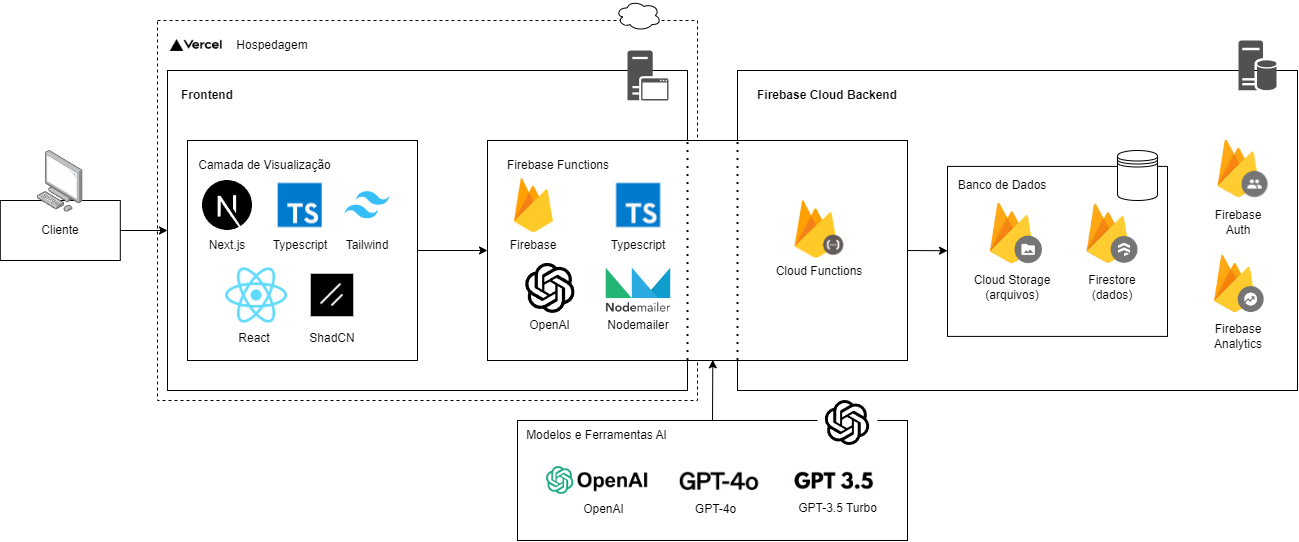
\includegraphics[width=15cm]{img/infra-model.png}
 	    \fonte{Os autores.}
\end{figure}

\subsection{Front-end}
O Front-end é a interface da aplicação, construída com Next.js, um framework React que oferece otimizações de desempenho e server-side rendering para uma experiência de usuário mais rápida e fluida. No desenvolvimento da interface, são empregadas as seguintes tecnologias:

\begin{itemize}
    \item \textbf{Tailwind CSS} \newline
Tailwind CSS é uma ferramenta utilizada para a estilização da aplicação. Ele adota uma abordagem de "utility-first", o que significa que as classes CSS são utilizadas diretamente no HTML para estilizar os elementos. Isso proporciona uma experiência de desenvolvimento mais rápida e consistente, além de facilitar a manutenção do código.

    \item \textbf{ShadCN} \newline
ShadCN é uma coleção de componentes prontos que podem ser importados e customizados dentro do código. Esses componentes são escritos em Typescript e Tailwind CSS. Ele não é considerado uma biblioteca, já que é uma extensão do Radix, outra biblioteca de estilização para Javascript.

    \item \textbf{Moment} \newline
Moment.js é uma biblioteca popular para manipulação de datas e horas em JavaScript. Ela oferece uma ampla gama de funcionalidades para formatação, análise e manipulação de datas, tornando mais fácil trabalhar com informações temporais na aplicação.

    \item \textbf{Nodemailer} \newline
Nodemailer é uma biblioteca utilizada para enviar e-mails através de Node.js. Ela oferece uma interface simples e flexível para o envio de e-mails, permitindo configurar facilmente o servidor de e-mail, criar templates personalizados e enviar mensagens de forma assíncrona.

    \item \textbf{Framer Motion} \newline
Framer Motion é uma biblioteca de animações para React que facilita a criação de animações fluidas e responsivas em componentes da interface. Ela oferece uma API declarativa e intuitiva para definir animações de entrada, saída e transição, além de suportar gestos e interações do usuário.

    \item \textbf{PDF Viewer} \newline
PDF Viewer é uma biblioteca Javascript projetada especificamente para a leitura de arquivos em formato PDF enviados pelos usuários, dentro do NodeJS. Com uma série de ferramentas avançadas, oferece uma experiência de visualização personalizada e intuitiva desses documentos.

    \item \textbf{Google Generative AI} \newline
A biblioteca Google AI JavaScript SDK permite que os desenvolvedores usem os modelos de IA generativos de última geração do Google (como o Gemini) para criar recursos e aplicativos com tecnologia de IA.

    \item \textbf{Bibliotecas do Firebase} \newline
Dentro do Front-end, são utilizadas diversas bibliotecas do Firebase para interação com o Back-end e execução de funcionalidades como autenticação, armazenamento de dados e comunicação em tempo real. Algumas das bibliotecas comumente utilizadas incluem:
\begin{itemize}
    \item \textbf{firebase}
    \item \textbf{firebase-admin}
    \item \textbf{firebase-functions}
    \item \textbf{firebase-tools}
\end{itemize}

Essas bibliotecas fornecem uma integração simplificada entre o Front-end e o Back-end, permitindo o desenvolvimento de uma aplicação robusta e interativa.

\end{itemize}

\subsection{Back-end}
Para o Back-end, é utilizado Firebase, que fornece serviços de banco de dados, armazenamento, autenticação e hospedagem, entre outros, de forma simplificada. O Firebase permite uma configuração rápida e fácil, facilitando o desenvolvimento e a viabilização do projeto.
Dentro da plataforma do Firebase, são utilizadas as seguintes funcionalidades:

\begin{itemize}
\item \textbf{Firebase Auth} \newline
Para autenticação de usuários, permitindo login com e-mail, redes sociais, entre outros métodos.
\item \textbf{Firebase Firestore} \newline
Para armazenamento e gerenciamento de dados em tempo real, oferecendo um banco de dados NoSQL escalável e altamente disponível.
\item \textbf{Firebase Storage} \newline
Para armazenamento de arquivos, como imagens e vídeos, diretamente na infraestrutura do Firebase.
\end{itemize}

\subsection{Banco de dados}
O banco de dados da aplicação está contido nos serviços oferecidos pelo Firebase Realtime Database e Firestore, que são bancos de dados NoSQL escaláveis e altamente disponíveis. A comunicação entre as camadas, API externas e com o cliente são realizadas através do Protocolo HTTP e chamadas REST.
O banco de dados é estruturado da seguinte maneira, a fim de suportar a gestão das informações dentro da plataforma:

\begin{itemize}
    \item \textbf{Tabela users}
    
    \begin{itemize}
    \item \textbf{fullname:} Armazena o nome completo do usuário.
    \item \textbf{email:} Guarda o endereço de e-mail do usuário.
    \item \textbf{document:} Pode armazenar o documento de identificação do usuário, como CPF. 
    \item \textbf{noticeid:} Chave estrangeira que faz referência ao edital (notice) associado ao usuário.
    \end{itemize}
    
    \item \textbf{Tabela tasks}
    
    \begin{itemize}
    \item \textbf{title:} Título da tarefa.
    \item \textbf{description:} Descrição detalhada da tarefa.
    \item \textbf{contentid:} Chave estrangeira que referencia o conteúdo (content) associado à tarefa. 
    \item \textbf{difficultyid:} Chave estrangeira que referencia o nível de dificuldade da tarefa. 
    \item \textbf{hasfinished:} Indica se a tarefa foi concluída ou não.
    \item \textbf{userid:} Chave estrangeira que faz referência ao usuário que criou a tarefa. 
    \item \textbf{dayofweek:} Dia da semana em que a tarefa deve ser realizada.
    \item \textbf{startat:} Horário de início da tarefa.
    \item \textbf{finishat:} Horário de término da tarefa.
    \end{itemize}
    
    \item \textbf{Tabela difficulties}
    
    \begin{itemize}
    \item \textbf{name:} Nome do nível de dificuldade.
    \item \textbf{displayname:} Nome de exibição do nível de dificuldade.
    \end{itemize}
    
    \item \textbf{Tabela subjects (matérias)}
    \begin{itemize}
    \item \textbf{name:} Nome da matéria.
    \item \textbf{noticeid:} Chave estrangeira que faz referência ao edital (notice) associado à matéria.
    \end{itemize}
    
    \item \textbf{Tabela contents}
    \begin{itemize}
    \item \textbf{subjectid:} Chave estrangeira que referencia a matéria (subject) associada ao conteúdo. 
    \item \textbf{text:} Texto do conteúdo, que pode conter informações relevantes para estudo.
    \end{itemize}
    
    \item \textbf{Tabela notices (editais)}
    \begin{itemize}
    \item \textbf{name:} Nome do cargo ou edital.
    \item \textbf{filesrc:} Caminho para o arquivo do edital. 
    \item \textbf{userid:} Usuário que fez o upload do edita.
    \end{itemize}
    
\end{itemize}

Este modelo de banco de dados é projetado para permitir a associação de usuários a tarefas específicas, associadas a conteúdos de estudo e matérias específicas relacionadas aos editais. A inclusão de um nível de dificuldade (na tabela difficulties) proporciona uma maneira de classificar a complexidade das tarefas, enquanto a tabela notices permite o armazenamento e acesso aos editais relacionados aos estudos.

 \begin{figure}[!htb]
 	    \centering
 	    \caption{\label{logo}Modelo de classes do banco de dados}
 	    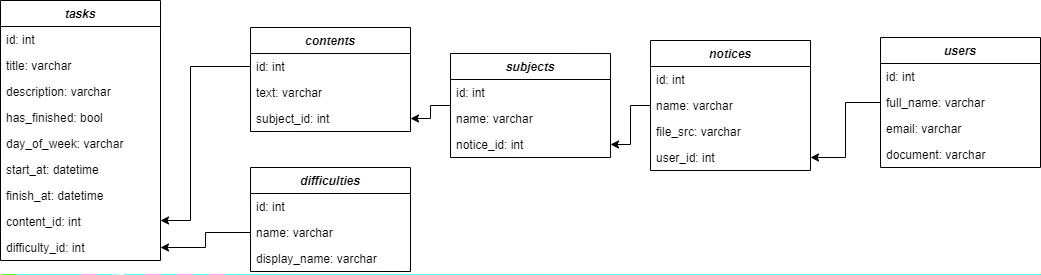
\includegraphics[width=15cm]{img/db-model.png}
 	    \fonte{Os autores.}
\end{figure}
\FloatBarrier

\subsection{Integrações}
Para a interpretação dos conteúdos pragmáticos dentro dos editais, faremos uso e customização dos modelos de inteligência artificial fornecidos pelo Google Gemini. O Gemini, anteriormente conhecido como Bard, é um chatbot desenvolvido pelo Google, baseado na família de modelos de linguagem LaMDA.
No contexto específico de nossa plataforma, contamos com dois modelos treinados para desempenhar funções cruciais:

\begin{itemize}
\item \textbf{Interpretação de Conteúdo de Edital e Geração de Matérias} \newline
Este modelo é encarregado de interpretar o conteúdo pragmático após a filtragem do edital fornecido pelo usuário. Ele irá identificar e extrair as matérias que serão cobradas no concurso, populando assim o banco de dados.

\item \textbf{Interpretação de Matérias e Geração de Tarefas e Rotinas de Estudo} \newline
 Com o banco de dados já contendo as matérias identificadas, este modelo entra em ação para gerar tarefas e rotinas de estudo personalizadas. Recebendo como entrada as matérias e conteúdos que o usuário ainda precisa estudar, ele irá gerar um cronograma de estudo detalhado, distribuindo as tarefas ao longo da semana de acordo com as necessidades e preferências do usuário.
\end{itemize}

Essas integrações permitem uma abordagem mais eficiente e personalizada no processo de estudo para concursos, aproveitando o poder dos modelos de linguagem avançados fornecidos pelo Google Gemini.

\subsection{Versionamento de Código}
O versionamento de código é uma prática fundamental no desenvolvimento de software, permitindo o controle e gerenciamento das alterações feitas ao longo do tempo em um projeto. Para isso, utilizaremos o GitHub como plataforma de versionamento, que oferece uma série de recursos poderosos para colaboração e controle de versões. No nosso ambiente de desenvolvimento, teremos um repositório principal hospedado no GitHub:

\textbf{Repositório do Front-end e Functions do Firebase:} \newline
Este repositório conterá o código-fonte do Front-end desenvolvido com Next.js, bem como as functions do Firebase utilizadas no Back-end. Será organizado de forma a separar claramente os diretórios relacionados ao Front-end e às functions do Firebase, mantendo uma estrutura de pastas intuitiva e coesa.

\textbf{Estratégia de Versionamento: Gitflow} \newline
Para gerenciar as diferentes etapas de desenvolvimento e garantir uma colaboração eficiente entre os membros da equipe, adotaremos a estratégia de versionamento Gitflow. Essa abordagem define um modelo de fluxo de trabalho baseado em branches, que facilita a organização das funcionalidades em desenvolvimento, testes e produção.
Principais Branches:

\begin{itemize}
\item \textbf{Main (ou Master):} Esta branch representa a versão estável e de produção do código. Todo o código que está pronto para ser implantado em ambiente de produção é mesclado nesta branch.

\item \textbf{Develop:} Esta branch é onde o desenvolvimento ativo ocorre. É a branch de integração para novas funcionalidades e correções de bugs. Todo o desenvolvimento é feito a partir desta branch.

\item \textbf{Feature Branches:} Para cada nova funcionalidade ou tarefa, uma nova branch de feature é criada a partir da branch develop. Esta branch é utilizada para implementar a funcionalidade de forma isolada, antes de ser integrada de volta à branch develop.
\end{itemize}
 
Adotando essa estratégia de versionamento com o Gitflow, garantimos um desenvolvimento organizado, facilitando a colaboração entre os membros da equipe e mantendo um histórico claro e estruturado das alterações feitas no código-fonte ao longo do tempo.

\subsection{Infraestrutura}
Para hospedagem, optaremos por utilizar os serviços especializados de hospedagem da Vercel para o Front-end e do Firebase para o Back-end customizado.

\textbf{Hospedagem do Front-end} \newline
A Vercel oferece um serviço de hospedagem altamente escalável e otimizado para aplicações Front-end, como o nosso desenvolvido com Next.js. Utilizando a plataforma da Vercel, podemos implantar e hospedar facilmente nosso Front-end, garantindo uma experiência de usuário rápida e confiável.

\textbf{Hospedagem do Back-end no Firebase} \newline
O Firebase oferece por padrão a hospedagem de seus serviços diretamente em sua plataforma, eliminando a necessidade de recorrer a soluções terceirizadas para essa finalidade. Essa integração nativa proporciona uma infraestrutura completa e integrada, capaz de suportar todas as necessidades de nossa aplicação de forma eficiente e escalável.

\subsection{Escalabilidade}
Tanto a Vercel quanto o Firebase oferecem opções de escalabilidade conforme as necessidades do projeto. No caso da Vercel, podemos facilmente escalar nossa aplicação Front-end de acordo com o aumento da demanda de tráfego. Já o Firebase, além de oferecer hospedagem escalável, também permite dimensionar automaticamente o banco de dados e outros serviços conforme necessário.

\subsection{Plano de Upgrade}
Inicialmente, faremos uso dos planos gratuitos oferecidos pela Vercel. Já no Firebase, iremos utilizar o plano “pay-as-you-go”, ou seja, o faturamento da conta será de acordo com o uso da plataforma. Optamos por esse plano pois ele nos disponibiliza o uso das Functions, que será essencial para a funcionalidade da nossa plataforma.
Conforme a aplicação crescer e a demanda aumentar, poderemos considerar a migração para planos pagos que oferecem recursos adicionais e maior capacidade de processamento. Essa decisão será tomada conforme a evolução do projeto e as necessidades específicas que surgirem ao longo do tempo.


\begin{comment}

\chapter{Migrar do site}
% https://www.overleaf.com/learn/latex/Articles/How_to_write_in_Markdown_on_Overleaf
\todo[inline]{Coloquei como outro arquivo  pds.md para ficar mais facil de ajustar e remover o que precisar conforme formos ajustando}
\markdownInput{pds.md}

\end{comment}


% ----------------------------------------------------------
% Finaliza a parte no bookmark do PDF
% para que se inicie o bookmark na raiz
% e adiciona espaço de parte no Sumário
% ----------------------------------------------------------
\phantompart

% ----------------------------------------------------------
% ELEMENTOS PÓS-TEXTUAIS
% ----------------------------------------------------------
\postextual
% ----------------------------------------------------------

% ----------------------------------------------------------
% Referências bibliográficas
% ----------------------------------------------------------
\bibliography{referencias}

% ----------------------------------------------------------
% Glossário
% ----------------------------------------------------------
%
%
\ifdef{\printnoidxglossary}{
    \addcontentsline{toc}{chapter}{GLOSSÁRIO}
    \printnoidxglossary[style=glossario]
    %\printglossaries
}{}

%% ----------------------------------------------------------
% Apêndices
% Documentos gerados pelo próprio autor
% ----------------------------------------------------------

% ---
% Inicia os apêndices
% ---
\begin{apendicesenv}

% Imprime uma página indicando o início dos apêndices
\partapendices

% ----------------------------------------------------------
\chapter{Quisque libero justo}
% ----------------------------------------------------------

\lipsum[1-2]

% ----------------------------------------------------------
\chapter{Nullam elementum urna vel imperdiet sodales elit ipsum pharetra ligula
ac pretium ante justo a nulla curabitur tristique arcu eu metus}
% ----------------------------------------------------------
\lipsum[3-5]

\end{apendicesenv}
% ---

%% ----------------------------------------------------------
% Anexos
% Documentos gerados por outros autores
% ----------------------------------------------------------

% ---
% Inicia os anexos
% ---
\begin{anexosenv}

% Imprime uma página indicando o início dos anexos
\partanexos

% ---
\chapter{Manual todonotes}
\label{manual-todonotes}
% ---
\index{pdf}
% arquivo completo
\includepdf[pages=-,frame=true]{anexos/todonotes.pdf}

% ---
\chapter{Manual pdfpages(parcial)}
% ---
\index{pdf}
% somente algumas páginas
\includepdf[pages=1-3,frame=false]{anexos/pdfpages.pdf}

% ---
\chapter{Manual acronym(parcial)}
% ---
\index{pdf}
% somente algumas páginas
\includepdf[pages=1-3,frame=false]{anexos/acronym.pdf}


% ---
\chapter{Cras non urna sed feugiat cum sociis natoque penatibus}
% ---

\lipsum[1]



\end{anexosenv}



%---------------------------------------------------------------------

\end{document}